\documentclass{jreport}
\usepackage{amsmath,amsthm,amssymb}
\usepackage{thmtools}
\usepackage[dvipdfmx]{graphicx}
\usepackage{float}
\usepackage{subfig}
\usepackage{caption}
\usepackage{color}
\usepackage{geometry}
\usepackage{algorithm,algpseudocode}
\usepackage{minted}
\usepackage{multicol}
\usepackage{enumerate}
\usepackage{verbatim}
\usepackage{hyperref}
\usepackage{mytitle}


\renewcommand{\thesubsection}{(\alph{subsection})}

\graphicspath{{../res/figure/}{../res/plot-the/}}
\makeatletter
\def\input@path{{../res/figure/}{../res/graph/}{../res/table-the/}}
\makeatother

% define command for pandoc
\providecommand{\tightlist}{\setlength{\itemsep}{0pt}\setlength{\parskip}{0pt}}

% setting margin
\newgeometry{tmargin=2cm,lmargin=2cm,rmargin=2cm,bmargin=2cm}

% adding new symbol (vrectangle and vrectangleblack)
\DeclareFontEncoding{LS1}{}{}
\DeclareFontSubstitution{LS1}{stix}{m}{n}
\DeclareSymbolFont{symbolsstix}{LS1}{stixscr}{m}{n}
\DeclareMathSymbol{\vrectangleblack}{\mathord}{symbolsstix}{"C5}
\DeclareMathSymbol{\vrectangle}{\mathord}{symbolsstix}{"C6}

% add math operator
\DeclareMathOperator*{\argmin}{\arg\!\min}
\DeclareMathOperator*{\argmax}{\arg\!\max}

% theorem preference
\declaretheoremstyle[
  spaceabove=1ex, 
  numbered=yes,
  headfont=\bfseries,
  headpunct=,
  bodyfont=\normalfont,
  spacebelow=1ex,
]{mythmstyle}
\declaretheorem[
  parent=chapter,style=mythmstyle,qed=$\vrectangle$,title=定義,
]{definition}
\declaretheorem[
  style=mythmstyle,sibling=definition,qed=$\vrectangle$,title=例,
]{example}
\declaretheorem[
  style=mythmstyle,sibling=definition,title=補題,
]{lemma}
\declaretheorem[
  style=mythmstyle,sibling=definition,qed=$\vrectangle$,title=補題,
]{lemma-without-proof}
\declaretheorem[
  style=mythmstyle,sibling=definition,title=定理,
]{theorem}
\declaretheorem[
  style=mythmstyle,sibling=definition,qed=$\vrectangle$,title=定理,
]{theorem-without-proof}
\declaretheorem[
  style=mythmstyle,sibling=definition,title=系,
]{collary}
\declaretheorem[
  style=mythmstyle,sibling=definition,qed=$\vrectangle$,title=系,
]{collary-without-proof}
\declaretheorem[
  style=mythmstyle,sibling=definition,qed=$\vrectangle$,title=予想,
]{conjecture}
\renewcommand{\proofname}{\normalfont{[\,証明\,]}\nopunct}
\renewcommand{\qedsymbol}{$\vrectangleblack$}

% algorithm preference
\renewcommand{\listalgorithmname}{アルゴリズムリスト}
\renewcommand{\thealgorithm}{\arabic{chapter}.\arabic{algorithm}}
\makeatletter
\renewcommand{\ALG@name}{アルゴリズム}
\@addtoreset{algorithm}{chapter}
\makeatother

% minted preference
\usemintedstyle{friendly}

% bibtex preference
\renewcommand{\bibname}{参考文献}
\bibliographystyle{junsrt}


\title{一般化ムーアグラフの探索の\\高効率化と高速化}
\author{里谷 佳紀}
\date{\today}
%\reportname{特 別 研 究 報 告 書}
\reportname{卒業論文}
\department{岡山大学工学部情報系学科}
\supervisor{高橋 規一}

\begin{document}

\maketitle


近年の急速なWebアプリケーションの発展に伴いデータセンタが注目されている.
データセンタではスイッチの相互接続による計算機ネットワークが利用されている.
スイッチの接続構造は一般に無向正則グラフでモデル化される.
ネットワークの性能はグラフの何らかの指標と関連しており,
特にデータ通信の遅延は平均頂点間距離と密接な関係をもつ.
そのため,平均頂点間距離の小さい無向正則グラフの構築は
低遅延なネットワークの構築のための重要な課題である.

平均頂点間距離が理論的下界と一致する正則グラフは一般化ムーアグラフと呼ばれる.
一般化ムーアグラフが存在するか否かは頂点数と次数の組合せに依存することが
知られているが,存在するための頂点数と次数に関する条件は完全には解明されていない.
現在まで,指定された頂点数と次数をもつ一般化ムーアグラフを探索する方法が
いくつか提案されてきた.
しかし,それらの方法には,頂点数と次数の任意の組に対応できない,
一般化ムーアグラフの性質を十分に利用していない,といった問題がある.

そこで,本研究は,頂点数と次数の任意の組に対応し,その性質を利用して
効率的に一般化ムーアグラフを探索する方法を提案し,その有効性を実験で検証する.
提案法は,全探索を基本として,初期グラフの制限や探索木の枝刈りによって
探索を効率的に行うものである.実験により,全域木から探索を開始することと,
直径の下界を用いた枝刈りが一般的に有効であることを示す.

\tableofcontents

\chapter{序論}
近年,Webアプリケーションの発展により,ユーザの活動によって生み出される膨大な
データの収集と活用が大いに注目されている.それを実現する技術の一つに,
データセンターが挙げられる.データセンターにはサーバが多数存在し,それぞれの
サーバがスイッチと接続し,さらにスイッチが相互に接続してネットワークを形成している
\cite{Greenberg2009,Al-Fares2008}.
ネットワークの性能はトポロジ(スイッチの接続構造)によって
変化する.最近,注目されるトポロジの一つにランダムトポロジがある
\cite{Singla2011,Koibuchi2012}.このトポロジは,Fat-Tree\cite{Al-Fares2008}
などの従来のトポロジと比べてスケーラビリティで優れているなどの特徴がある
\cite{Singla2011}.
その中でも,低遅延性はデータセンタのスループットに直結する重要な特性である.

このことから,低遅延なネットワークの構築が重要であることが分かる.
ネットワークを,スイッチを頂点とみなしたグラフで表現するとき,遅延は
は平均頂点間距離と呼ばれる値と関連する.現在まで,
平均頂点間距離が小さいグラフの構築に関する研究が行われてきた.
2015年,藤田らは,辺の入れ替えを繰り返しながら
グラフの平均頂点間距離を小さくする方法を開発した\cite{Fujita2015}.
ところが,この方法では局所解に陥ることが多く,平均頂点間距離が最小である
グラフを発見することが困難である.

一方で,1973年,Cerfらは,平均頂点間距離が小さい正則グラフとして一般化ムーアグラフを
提案し\cite{Cerf1973},翌年に一般化ムーアグラフの平均頂点間距離が
同じ頂点数と次数の正則グラフの中で下界であることを導出した\cite{Cerf1974Lower}.
一般化ムーアグラフを求める方法はいくつか知られている.
2004年,Sampelsは頂点推移グラフの中に一般化ムーアグラフが存在することを応用した
方法を開発した\cite{Sampels2004}.しかし,この方法では,任意の頂点数と次数の
一般化ムーアグラフを求めることはできない.
2016年,山本らは,佐藤らの正則グラフを列挙する方法\cite{Sato2008}を応用し,
途中で一般化ムーアグラフが発見されるまで列挙を繰り返す方法を開発した
\cite{Yamamoto2016}.
しかし,この方法は,一般化ムーアグラフがもつ性質を利用して効率的に探索できて
いないと言える.

そこで,本研究は,与えられた頂点数と次数の一般化ムーアグラフの
探索の効率的な方法の提案と,その方法の有効性の検証を目的とする.
まず,一般化ムーアグラフについて,その性質を説明した後,
深さ優先探索をベースにした探索アルゴリズムを示す.
その後,探索空間の削減による効率化の手法を提案し,その効果を検証する.
具体的には,探索の初期状態の変更と枝刈りの導入である.



\chapter{準備}
\label{chap:preliminary}
本章では,後の章に向けての準備をする.はじめに,グラフ理論の基本事項を説明する.
頂点間距離や直径などを含む.次に,Cerfらが提案した一般化ムーアグラフの
定義を与え,いくつかの性質を示す.これらの性質は,一般化ムーアグラフを
探索する方法に用いるもので,極めて重要である.

\section{グラフ理論の基本事項}
\label{sect:basic-graph-theory}
グラフ理論の基本事項を,\cite{Diestel2000}の記号に則り説明する.
グラフ理論の基礎を理解している読者は\ref{sect:generalized-moore-graph}節まで
読み飛ばしても差し支えない.

\textbf{グラフ}とは,二つの集合$V$と$E$の組$G=(V,E)$で,$E$は
$E\subseteq[V]^2$つまり,$V$から重複なく元を2個取り出した集合の部分集合である.
$V$を\textbf{頂点集合}とよび,その元を\textbf{頂点}とよぶ.
また,頂点集合の大きさ$|V|$を\textbf{頂点数}とよぶ.
$E$を\textbf{辺集合}とよび,その元を\textbf{辺}とよぶ.
後で示すように,グラフを図示する際,頂点は丸や点で,辺は頂点を結ぶ線で
表されることが多い.

頂点$v$と辺$e$が\textbf{接続する}とは,$v\in e$つまり,$e$の端点に$v$が
属することをいう.頂点$v$と頂点$w$が\textbf{隣接する}とは,$\{v,w\}$が
辺集合に属することをいう.

グラフ$G$上の頂点$v$に対して,その頂点と隣接している頂点の数を
\textbf{次数}と呼び,$d_G(v)$あるいは$d(v)$と記す.
すべての頂点について,その次数が一定のグラフを\textbf{正則グラフ}と呼ぶ.

\textbf{経路}$P$とは,$P=(V,E)$のグラフで,
\[ V=\{x_0,x_1,\ldots,x_k\},\:
E=\{\{x_0,x_1\},\{x_1,x_2\},\ldots,\{x_{k-1},x_k\}\}\]
を満たす$V$と$E$の組である.このときの辺の数を経路の\textbf{長さ}あるいは
\textbf{経路長}という.長さが2以上の閉路$P$に対して,その両端の頂点を
隣接させたグラフを\textbf{閉路}という.つまり,閉路$C=(V,E)$とは,
\[ V=\{x_0,x_1,\ldots,x_{k-1}\},\:
E=\{\{x_0,x_1\},\{x_1,x_2\},\ldots,\{x_{k-2},x_{k-1}\},\{x_{k-1},x_0\}\}\]
を満たす,$k\geq0$のグラフである.閉路$C$の辺の数あるいは頂点の数を,
閉路の\textbf{長さ}あるいは\textbf{閉路長}とよぶ.

グラフ$G$上の頂点$v$と$w$について,$v$と$w$を結ぶ最短の経路の長さを$v$と$w$の
\textbf{頂点間距離}とよび,$d_G(v,w)$あるいは$d(v,w)$で表す.
$v$と$w$を結ぶ経路が存在しないとき,$d(v,w):=\infty$と定義する.
経路の対称性より,$d(v,w)=d(w,v)$である.すべての二頂点の組合せに対する
頂点間距離の平均値と最大値をそれぞれ\textbf{平均頂点間距離}と\textbf{直径}
という.

\begin{example}
  図\ref{fig:graph-example}にグラフの例を示す.
  頂点集合は
  $\{u,v,w,x,y,z\}$
  で,辺集合は
  $\{(u,w),(v,x),(w,x),(w,y),(x,z),(y,z)\}$
  である.次数は,それぞれの頂点に対して,
  $d(u)=1,\,d(v)=1,\,d(w)=3,\,d(x)=3,\,d(y)=2,\,d(z)=2$
  である.グラフには,長さ4の閉路
  $\{w,x,z,y\}$
  が存在する.頂点間距離は次のとおり.
  \begin{equation*}
    \begin{aligned}
      d(u,v)=3&\:&d(u,w)=1&\:&d(u,x)=2&\:&d(u,y)=2&\:&d(u,z)=3 \\
      &\:&d(v,w)=2&\:&d(v,x)=1&\:&d(v,y)=3&\:&d(v,z)=2 \\
      &\:&&\:&d(w,x)=1&\:&d(w,y)=1&\:&d(w,z)=2 \\
      &\:&&\:&&\:&d(x,y)=2&\:&d(x,z)=1 \\
      &\:&&\:&&\:&&\:&d(y,z)=1 \\
    \end{aligned}
  \end{equation*}
  平均頂点間距離は,頂点間距離の値の平均を求めると,$1.8$である.
  直径は,頂点間距離の値の最大値なので,$3$である.
  \begin{figure}
    \centering
    \input{graph-example.pdf_tex}
    \caption{グラフの例}
    \label{fig:graph-example}
  \end{figure}
\end{example}

\section{一般化ムーアグラフ}
\label{sect:generalized-moore-graph}
本節では一般化ムーアグラフを定義する.
さらに,これが満たすいくつかの性質を示す.

\begin{definition}[Cerf et.al., 1973\,\cite{Cerf1973}]
  \label{def:generalized-moore-graph}
  次の性質が成り立つ頂点数$n$,次数$k$の正則グラフを
  \textbf{一般化ムーアグラフ}(\textbf{Generalized Moore graph})とよぶ.

  すべての頂点$v$について,$v$から$i$離れた頂点の数
  $c_i = \lvert\{ w\,|\,d(v,w) = i , w\in V \}\rvert$について,
  \begin{equation}
    \label{eq:gmg-verts-dist}
    \begin{aligned}
      c_i =
      \begin{cases}
        k(k-1)^{i-1} & 1\leq i\leq Q \\
        R & i = Q+1 \\
        0 & Q+2\leq i \leq n-1
      \end{cases}
    \end{aligned}
  \end{equation}
  であること.ただし,
  \begin{align}
    Q(n,k)&=\max\{q|n-1-\sum_{i=1}^{q}k(k-1)^{i-1}\geq 0\}\label{eq:gmg-q} \\
    R(n,k)&=n-1-\sum_{i=1}^{Q(n,k)}k(k-1)^{i-1}\label{eq:gmg-r}
  \end{align}
  とする.
\end{definition}
\begin{example}
  図\ref{fig:gmg-example}に示したグラフを考える.
  $Q(12,3)$と$R(12,3)$はそれぞれ,
  \begin{align*}
    Q(12,3) &= \max\{q | 12-1-\sum_{i=1}^{q}3\cdot2^{i-1} \geq 0\} = 2 \\
    R(12,3) &= 12 - 1 - \sum_{i=1}^{Q(12,3)}3\cdot2^{i-1} = 2
  \end{align*}
  である.このグラフの頂点$1$に着目する.頂点$1$からの距離によって,
  残りの頂点を分類する.
  \begin{enumerate}
  \item 頂点$1$からの距離が$1$の頂点は$\{2,3,4\}$
  \item 頂点$1$からの距離が$2$の頂点は$\{5,6,7,8,9,10\}$
  \item 頂点$1$からの距離が$3$の頂点は$\{11,12\}$
  \end{enumerate}
  である.$1$からの距離が$i$の頂点数$c_i$は,
  \begin{align*}
  c_1 &= 3\cdot2^0 = 3 & \\
  c_2 &= 3\cdot2^1 = 6 & \\
  c_3 &= R(12,3) = 2 & \\
  c_i &= 0 & (i>3)
  \end{align*}
  となるので,式\ref{eq:gmg-verts-dist}で示した距離と頂点数の
  関係を満たす.同様に,他のすべての頂点について,上述の距離と頂点数の関係を
  満たす.よって,このグラフは一般化ムーアグラフである.
  \begin{figure}
    \centering
    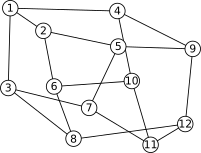
\includegraphics{gmg-example.pdf}
    \caption{頂点数12,次数3の一般化ムーアグラフの例}
    \label{fig:gmg-example}
  \end{figure}
\end{example}
以下,頂点数$n$,次数$k$の一般化ムーアグラフを$M(n,k)$と記し,
$Q(n,k)$と$R(n,k)$をそれぞれ式\ref{eq:gmg-q}と式\ref{eq:gmg-r}のとおりとする.
頂点数と次数が文脈から明らかな場合は省略してそれぞれ$M,Q,R$と表す.

一般化ムーアグラフの頂点間距離の総和を求め,これが正則グラフの頂点間距離の総和の
下界であることを示す.
\begin{theorem}[Cerf et.al., 1974\,\cite{Cerf1974Lower}]
  \label{thm:gmg-lower-bound}
  $M(n,k)$の頂点間距離の総和は,
  \begin{equation}
    \label{eq:gmg-lb}
    S(n,k) = \sum_{(s,t)\in V\times V}d(s,t) =
    n \left[\ \sum^{Q}_{i=1}ik(k-1)^{i-1} + (Q+1)R\ \right]
  \end{equation}
  で与えられる.これは,正則グラフの頂点間距離の総和の下界である.
\end{theorem}
\begin{proof}
  ある頂点$v$から頂点$w(\neq v)$との距離の総和を次式で表す.
  \begin{equation}
    \label{eq:gmg-lb-1}
    \sum_{i=1}^{n-1}i c_i
  \end{equation}
  ここで,$c_i$は$v$との距離が$i$の頂点の個数とする.
  一般化ムーアグラフの場合,$c_i$は式\ref{eq:gmg-verts-dist}で与えられる.
  そのため,式\ref{eq:gmg-lb-1}から,
  \begin{align}
      \sum_{i=1}^{n-1}ic_i
      &=\sum_{i=1}^{Q}ic_i+(Q+1)c_{Q+1}+\sum_{i=Q+2}^{n-1}ic_i \nonumber\\
      &=\sum_{i=1}^{Q}ik(k-1)^{i-1}+(Q+1)R
      \label{eq:gmg-lb-2}
  \end{align}
  が得られる.これは一つの頂点から他のすべての頂点への距離の総和を表すので,
  式\ref{eq:gmg-lb-2}を$n$倍すると,式\ref{eq:gmg-lb}が得られる.

  次に,式\ref{eq:gmg-lb}が頂点間距離の総和の下界であることを示す.
  一般的な$c'_i$に対して,
  \begin{equation}
    \label{eq:gmg-lb-3}
    \sum_{i=1}^{n-1}i c_i \leq \sum_{i=1}^{n-1}i c'_i
  \end{equation}
  であることを証明する.
  $1\leq i\leq Q$の範囲で,$c_i$は最大なので次が得られる.
  \begin{equation}
    \label{eq:gmg-lb-4}
    \begin{aligned}
      c_i - c'_i
      \begin{cases}
        \geq 0 & 1\leq i\leq Q \\
        \lesseqgtr 0 & i = Q+1 \\
        \leq 0 & Q+2\leq i\leq n-1
      \end{cases}
    \end{aligned}
  \end{equation}
  $c_{Q+1}\geq c'_{Q+1}$と$c_{Q+1}\leq c'_{Q+1}$のふたつの場合について考える.
  \begin{enumerate}[(i)]
  \item $c_{Q+1}\geq c'_{Q+1}$のとき
  \end{enumerate}
  $c_{Q+1}\geq c'_{Q+1}$ならば$c_{Q+1}-c'_{Q+1}\geq0$となり,
  式\ref{eq:gmg-lb-4}より,
  \begin{equation}
    \label{eq:gmg-lb-5a}
    \begin{aligned}
      c_i-c'_i
      \begin{cases}
        \geq 0 & 1\leq i\leq Q+1 \\
        \leq 0 & Q+2\leq i\leq n-1
      \end{cases}
    \end{aligned}
  \end{equation}
  が成り立つ.$c_i$の定義より,次が成り立つ.
  \begin{equation}
    \label{eq:gmg-lb-6}
    \sum_{i=1}^{n-1}c_i = \sum_{i=1}^{n-1}c'_i = n-1
  \end{equation}
  式\ref{eq:gmg-lb-5a}と式\ref{eq:gmg-lb-6}より,
  \begin{equation}
    \label{eq:gmg-lb-7a}
    \begin{aligned}
      \sum_{i=1}^{Q+1}(c_i-c'_i) &= \sum_{i=1}^{Q+1}|c_i-c'_i| \\
      \sum_{i=Q+2}^{n-1}(c_i-c'_i) &= -\sum_{i=Q+2}^{n-1}|c_i-c'_i| \\
      \sum_{i=1}^{Q+1}|c_i-c'_i| &= \sum_{i=Q+2}^{n-1}|c_i-c'_i|
    \end{aligned}
  \end{equation}
  が得られる.式\ref{eq:gmg-lb-7a}を用いて,式\ref{eq:gmg-lb-8a}を考える.
  \begin{equation}
    \label{eq:gmg-lb-8a}
    \sum_{i=1}^{n-1}i(c_i-c'_i)=
    \sum_{i=1}^{Q+1}i|c_i-c'_i|-\sum_{i=Q+2}^{n-1}|c_i-c'_i|
  \end{equation}
  式\ref{eq:gmg-lb-8a}の第一項の上界は,式\ref{eq:gmg-lb-8a1}である.
  \begin{equation}
    \label{eq:gmg-lb-8a1}
    \sum_{i=1}^{Q+1}i|c_i-c'_i|\leq (Q+1)\sum_{i=1}^{Q+1}|c_i-c'_i|
  \end{equation}
  式\ref{eq:gmg-lb-8a}の第二項の下界は,式\ref{eq:gmg-lb-8a2}である.
  \begin{equation}
    \label{eq:gmg-lb-8a2}
    \sum_{i=Q+2}^{n-1}i|c_i-c'_i|\geq (Q+2)\sum_{i=Q+2}^{n-1}|c_i-c'_i|
  \end{equation}
  式\ref{eq:gmg-lb-8a1}と式\ref{eq:gmg-lb-8a2}より,次が成り立つ.
  \begin{align*}
    \sum_{i=1}^{n-1}i(c_i-c'_i)
    &\leq (Q+1)\sum_{i=1}^{Q+1}|c_i-c'_i|-(Q+2)\sum_{i=Q+2}^{n-1}|c_i-c'_i| \\
    &= (Q+1)\sum_{i=1}^{Q+1}|c_i-c'_i|-(Q+2)\sum_{i=1}^{Q+1}|c_i-c'_i| \\
    &= -\sum_{i=1}^{Q+1}|c_i-c'_i| \\
    &\leq 0
  \end{align*}
  ゆえに式\ref{eq:gmg-lb-3}が成り立つ.

  \begin{enumerate}[(i)]
    \setcounter{enumi}{1}
  \item $c_{Q+1}\leq c'_{Q+1}$の場合もほとんど同じである.
  \end{enumerate}
  $c_{Q+1}\leq c'_{Q+1}$ならば$c_{Q+1}-c'_{Q+1}\leq0$となり,
  式\ref{eq:gmg-lb-4}より,
  \begin{equation}
    \label{eq:gmg-lb-5b}
    \begin{aligned}
      c_i-c'_i
      \begin{cases}
        \geq 0 & 1\leq i\leq Q \\
        \leq 0 & Q+1\leq i\leq n-1
      \end{cases}
    \end{aligned}
  \end{equation}
  式\ref{eq:gmg-lb-5b}と式\ref{eq:gmg-lb-6}より,
  \begin{equation}
    \label{eq:gmg-lb-7b}
    \begin{aligned}
      \sum_{i=1}^{Q}(c_i-c'_i) &= \sum_{i=1}^{Q}|c_i-c'_i| \\
      \sum_{i=Q+1}^{n-1}(c_i-c'_i) &= -\sum_{i=Q+1}^{n-1}|c_i-c'_i| \\
      \sum_{i=1}^{Q}|c_i-c'_i| &= \sum_{i=Q+1}^{n-1}|c_i-c'_i|
    \end{aligned}
  \end{equation}
  が得られる.式\ref{eq:gmg-lb-7a}を用いて,次の式\ref{eq:gmg-lb-8b}を考える.
  \begin{equation}
    \label{eq:gmg-lb-8b}
    \sum_{i=1}^{n-1}i(c_i-c'_i)=
    \sum_{i=1}^{Q}i|c_i-c'_i|-\sum_{i=Q+1}^{n-1}|c_i-c'_i|
  \end{equation}
  式\ref{eq:gmg-lb-8b}の第一項の上界は,次の式\ref{eq:gmg-lb-8b1}である.
  \begin{equation}
    \label{eq:gmg-lb-8b1}
    \sum_{i=1}^{Q}i|c_i-c'_i|\leq Q\sum_{i=1}^{Q}|c_i-c'_i|
  \end{equation}
  式\ref{eq:gmg-lb-8b}の第二項の下界は,次の式\ref{eq:gmg-lb-8b2}である.
  \begin{equation}
    \label{eq:gmg-lb-8b2}
    \sum_{i=Q+1}^{n-1}i|c_i-c'_i|\geq (Q+1)\sum_{i=Q+1}^{n-1}|c_i-c'_i|
  \end{equation}
  式\ref{eq:gmg-lb-8b1}と式\ref{eq:gmg-lb-8b2}より,次が成り立つ.
  \begin{align*}
    \sum_{i=1}^{n-1}i(c_i-c'_i)
    &\leq Q\sum_{i=1}^{Q}|c_i-c'_i|-(Q+1)\sum_{i=Q+1}^{n-1}|c_i-c'_i| \\
    &= Q\sum_{i=1}^{Q}|c_i-c'_i|-(Q+1)\sum_{i=1}^{Q}|c_i-c'_i| \\
    &= -\sum_{i=1}^{Q}|c_i-c'_i| \\
    &\leq 0
  \end{align*}
  ゆえに式\ref{eq:gmg-lb-3}が成り立つ.
\end{proof}

\begin{example}
  再び$M(12,3)$について考える.$M(12,3)$の頂点間距離の総和は,
  式\ref{eq:gmg-lb}より,
  \[ 12\left[\sum_{i=1}^2i\cdot3\cdot(3-1)^{i-1}+(2+1)\cdot2\right]=
  12(3+12+6)=252\]
  である.ちなみに,図\ref{fig:gmg-example}に示したグラフの
  頂点間距離の総和を求めると,同じく252である.
\end{example}

次の性質は,一般化ムーアグラフが満たす構造的な特徴を示す.
後に説明する探索方法に用いる極めて重要な性質である.
\begin{theorem}
  \label{thm:gmg-geometric-property}
  ある正則グラフが一般化ムーアグラフであることの必要十分条件は,
  \begin{enumerate}[(a)]
  \item 長さ$2Q$以下の閉路を持たないこと
    \label{gmg-geom-a}
  \item 直径が$R=0$のときは$Q$,\hspace{1ex}$R>0$のときは$Q+1$であること.
    \label{gmg-geom-b}
  \end{enumerate}
  の二条件を同時に満たすことである.
\end{theorem}
\begin{proof}
  正則グラフの頂点数を$n$,次数を$k$とする.
  条件\ref{gmg-geom-a}を満たすならば,すべての頂点$v$に対して,
  $d(v,w)=i$なる頂点$w$の数$c'_i$は,$c'_i=k(k-1)^{i-1}(1\leq i\leq Q)$となる.
  また,条件\ref{gmg-geom-b}を満たすならば,$c'_i=0(Q+2\leq i)$である.
  これら二つを同時に満たすとき,
  \[ c'_{Q+1}=n-1-\sum_{i=1}^{Q}k(k-1)^{i-1}=R \]
  を満たす.よって,ある正則グラフが条件\ref{gmg-geom-a}と
  条件\ref{gmg-geom-b}を同時に満たすとき,それは$M(n,k)$である.

  逆を証明する.$c_i=k(k-1)^{i-1}(1\leq i\leq Q)$ならば,
  すべての頂点$v$について,頂点$w\,(d(v,w)=i<Q)$は,
  $k-1$個の頂点$x\,(d(v,x)=i+1)$と隣接する.
  従って,一般化ムーアグラフ$M(n,k)$には,長さ$2Q$以下の閉路は存在しない.
  また,$Q+2\leq i$(ただし,$R=0$の場合$Q+1\leq i$)の範囲で$c_i=0$なので,
  すべての頂点$v$について,$d(v,w)\geq Q+2$\hspace{.3ex}$(Q+1)$となるような
  頂点$w$は存在しない.従って,直径は$Q+1$\hspace{.3ex}$(Q)$である.
  よって,$M(n,k)$は条件\ref{gmg-geom-a}と条件\ref{gmg-geom-b}を
  同時に満たす.
\end{proof}
\begin{example}
  もう一度$M(12,3)$について考える.図\ref{fig:gmg-example}のグラフを
  \verb|igraph|ライブラリで解析する.図\ref{fig:gmg-example}の
  データとして,ファイル\verb|n12-d3-example.elist|に
  \begin{multicols}{4}
    \verbatiminput{n12-d3-example.elist}
  \end{multicols}
  が格納されているとする.ただし,辺のリストを4列で表しているが
  実際は1列である.プログラム
  \begin{minted}{python}
    from __future__ import print_function
    import igraph as ig
    G = ig.read('n12-d3-example.elist', 'edgelist') # データ読み込み
    print('diameter: ', G.diameter())               # 直径
    print('girth: ', G.girth())                     # 最小の閉路長
  \end{minted}
  を\verb|python|で実行すると,次が得られる.
  \begin{verbatim}
    diameter: 3
    girth: 5
  \end{verbatim}
  $Q=2,\,R=2$なので,このグラフは
  定理\ref{thm:gmg-geometric-property}の二条件を満たす.
\end{example}

最後に,一般化ムーアグラフの直径の式を与える.その前に,
式\ref{eq:gmg-q}を変形する.
\begin{lemma}
  \label{lem:gmg-q}
  \begin{equation}
    Q(n,k) = \left\lfloor
    \log_{k-1}\left(1+\frac{(n-1)(k-2)}{k}\right)\right\rfloor
  \end{equation}
\end{lemma}
\begin{proof}
  式\ref{eq:gmg-q}より,
  \begin{align}
    n &= 1 + \sum_{i=1}^Qk\cdot(k-1)^{i-1} + R \nonumber\\
    &= 1 + \frac{k\left((k-1)^{Q}-1\right)}{k-2} + R
    \label{eq:gmg-q-1}
  \end{align}
  が得られる.さらに変形して,
  \begin{align}
    (k-1)^Q &= 1+\frac{(n-R-1)(k-2)}{k} \nonumber\\
    Q &= \log_{k-1}\left(1+\frac{(n-R-1)(k-2)}{k}\right)
    \label{eq:gmg-q-2}
  \end{align}
  となる.ここで,式\ref{eq:gmg-q-2}の$R$を除去するために,
  次の関数$f$を考える.
  \begin{equation}
    \label{eq:gmg-q-3}
    f(n,k) = \log_{k-1}\left(1+\frac{(n-1)(k-2)}{k}\right)
  \end{equation}
  $f(n',k)=Q'$を満たす$n'$は,式\ref{eq:gmg-q-3}から,
  \[ n'=1+\sum_{i=1}^{Q'}k(k-1)^{i-1} \]
  と求められる.同様に,$f(n'',k)=Q'+1$を満たす$n''$は,
  \[ n''=1+\sum_{i=1}^{Q'+1}k(k-1)^{i-1} = n''+k(k-1)^{Q'} \]
  である.
  $0\leq R' < k(k-1)^{Q'}$なる$R'$について,$f(n'+R',k)$の値は,
  $\log_{k-1}$が単調増加関数であることに注意すると,
  \[ f(n',k) \leq f(n'+R',k) < f(n'',k) \]
  と範囲を定められる.ここで,$f(n',k)=Q'$,$f(n'',k)=Q'+1$なので,
  \begin{equation}
    \label{eq:gmg-q-4}
    Q' \leq f(n'+R',k) < Q'+1
  \end{equation}
  と書ける.よって,床関数を導入して,
  \[ Q(n,k) = \left\lfloor f(n,k)\right\rfloor
  = \left\lfloor\log_{k-1}\left(1+\frac{(n-1)(k-2)}{k}\right)\right\rfloor \]
  が成り立つ.
\end{proof}

\begin{theorem}
  \label{thm:gmg-diam}
  一般化ムーアグラフ$M(n,k)$の直径は,次で与えられる$\hat{Q}(n,k)$に等しい.
  \begin{equation}
    \hat{Q}(n,k)=
    \left\lceil\log_{k-1}\left(1+\frac{(n-1)(k-2)}{k}\right)\right\rceil
  \end{equation}
\end{theorem}
\begin{proof}
  $R=0$のとき,$\hat{Q}(n,k)=\lceil f(n,k)\rceil=Q(n,k)$が成り立つ.
  また,$0<R<k(k-1)^{Q(n,k)}$のとき,
  $\hat{Q}(n,k)=\lceil f(n,k)\rceil=Q(n,k)+1$となる.
  これら二つが成り立つので,定理\ref{thm:gmg-geometric-property}の直径
  の条件より,$\hat{Q}(n,k)$は一般化ムーアグラフ$M(n,k)$の直径の値と一致する.
\end{proof}
$\hat{Q}(v,k)$は,頂点$2$から順番に,頂点$1$から遠くなるように頂点を
配置した際の,頂点$1$と頂点$v$の距離$d(1,v)$の意味もある.
以降,$\hat{Q}(n,k)$について,文脈から$k$が明らかな場合は$\hat{Q}(n)$
と省略する.同じく,$n$と$k$が明らかな場合は,$\hat{Q}$と省略する.


\chapter{探索アルゴリズム}
\label{chap:basic-algorithm}
本章では,第\ref{chap:generalized-moore-graph}章で示した一般化ムーアグラフの
性質を利用して,与えられた頂点数と次数の一般化ムーアグラフを探索する基本的な
アルゴリズムを与える.これは後の章で探索空間を縮小する手法の比較対象となる.
まず,探索の初期状態と状態空間について説明した後,状態から新たな状態を生む
遷移について説明する.最後に,全体的なアルゴリズムを与える.

はじめに,ムーアバウンドを定義する.
\begin{definition}\rm
  \textbf{ムーアバウンド}(\textbf{Moore bound})とは,
  次数が$k$,直径が$D$の正則グラフの頂点数の上界で,次式で定義される.
  \begin{equation}
    n_{k,D} = 1 + \sum_{i=1}^Dk(k-1)^{i-1}
  \end{equation}
\end{definition}

ムーアバウンド$n_{k,D}$は次数$k$で$R=0,\ Q=D$の一般化ムーアグラフの頂点数に等しい.
ムーアバウンドを用いて探索の初期状態となる\textbf{初期グラフ}を定義する.

\begin{definition}\rm
  \label{def:basic-initial-graph}
  以下で定義されるグラフ$G_I$を\textbf{基本初期グラフ}とよぶ.
  基本初期グラフとは,次のグラフ$G_I$である.
  \begin{equation}
    \begin{aligned}
      \label{eq:basic-initial-graph}
      G_I&=(V,E) \\
      V&=\{1,\ldots,n\} \\
      E&=\{(1,2),\ldots,(1,k+1)\}\cup
      \{(\text{parent}(v),v)|v=k+2,\ldots,n-R\}
    \end{aligned}
  \end{equation}
  ただし
  \[\text{parent}(v)=
  \left\lceil\frac{v-n_{k,\hat{Q}(v)-1}}{k-1}\right\rceil+n_{k,\hat{Q}(v)-2}\]
  である.
\end{definition}

基本初期グラフの例を図\ref{fig:initial-tree-example}に示す.
基本初期グラフは頂点数$n-R$,最大次数$k$の平衡木と$R$個の孤立点で構成される.

次に,探索空間の基底となる辺の列である\textbf{候補辺列}を定義する.

\begin{definition}\rm
  \label{def:candidate-edges}
  候補辺列$\{e_i\}_{i\in\mathbb{N}}$とは,初期グラフ$G_I$に対して,
  $G_I$上で次数が$k$未満の頂点同士を隣接させる辺のうち,$G_I$に属していない
  辺の集合に順序を付加した列である.具体的には,次の式で定義される.
  \begin{equation}
    \{e_i\}_{i\in\mathbb{N}} =
    \{(v,w)\,|\,d_{G_I}(v)<k,d_{G_I}(w)<k,(v,w)\in[V]^2\}\setminus E(G_I)
  \end{equation}
  候補辺列に属する辺を\textbf{候補辺}とよぶ.
\end{definition}

一般化ムーアグラフの探索の探索空間は,候補辺の任意の個数の組合せと言える.
候補辺の例を図\ref{fig:feasible-edges-example}に破線で示す.

\begin{figure}
  \centering
  \begin{minipage}{.45\columnwidth}
    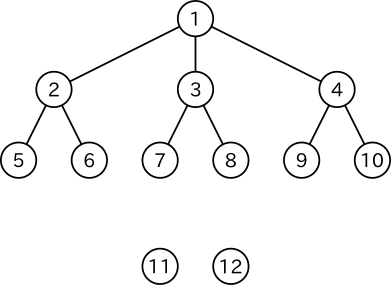
\includegraphics[width=\textwidth]{initial-tree-example.pdf}
    \captionof{figure}{基本初期グラフの例}
    \label{fig:initial-tree-example}
  \end{minipage}
  \hfill
  \begin{minipage}{.45\columnwidth}
    \def\svgwidth{\textwidth}
    \input{feasible-edges-example.pdf_tex}
    \captionof{figure}{候補辺の例(破線部分)}
    \label{fig:feasible-edges-example}
  \end{minipage}
\end{figure}

探索に用いる状態としてグラフ$G$と次に追加する候補辺の番号$i$の組を使う.
初期状態は$(G_I,1)$である.状態$(G,i)$が与えられたとき,
候補辺$e_i$を追加する遷移(\textbf{追加型遷移})と
追加しない遷移(\textbf{非追加型遷移})の動作を与える.
追加型遷移は与えられた状態$(G,i)$に対して状態$(G+e_i,i+1)$を返す.
また,非追加型遷移は与えられた状態$(G,i)$に対して状態$(G,i+1)$を返す.

遷移が適応可能な状態の条件を示す.その前に次の記号を定義する.
\begin{definition}\rm
  頂点$v$と候補辺列$\{e_i\}_{i\in\mathbb{N}}$について,$v$と接続している辺
  $e_i$の番号$i$の最小値と最大値をそれぞれ$\text{Enter}(v)$と
  $\text{Exit}(v)$とする.
  $\text{Enter}(v)$と$\text{Exit}(v)$の具体的な式は,次で与えられる.
  \begin{equation}
    \label{eq:frontier}
    \begin{aligned}
    \text{Enter}(v) &= \min\{i\,|\,v\in e_i\} \\
    \text{Exit}(v) &= \max\{i\,|\,v\in e_i\}
    \end{aligned}
  \end{equation}
\end{definition}

二種類の遷移それぞれについて,対象の候補辺以降の候補辺の選び方で
一般化ムーアグラフとなる見込みがあるかどうかを判定する方法を,
定理\ref{thm:gmg-geometric-property}より与える.

\begin{corollary-without-proof}\rm
  \label{coll:basic-add-transition}
  追加型遷移について,与えられたグラフを$G$,候補辺番号を$i$,候補辺を
  $e_i=\{v,w\}$,適応後のグラフを$G'$とする.$i$以降の候補辺の
  選び方次第で$G'$が一般化ムーアグラフとなる見込み
  があることとは,次の二条件の両方を満たすことである.
  \begin{enumerate}
  \item 次数条件:\ $d_G(v)<k$かつ,$d_G(w)<k$かつ,
    $\text{Exit}(x)=i$なる$x\in e_i$について$d_{G'}(x)=k$
  \item 閉路条件:\ $d_G(v,w)\geq2Q$
  \end{enumerate}
\end{corollary-without-proof}

閉路条件を満たすとき,辺が追加されてできる閉路の長さは少なくとも
$2Q+1$であり,定理\ref{thm:gmg-geometric-property}に反しない.

\begin{corollary-without-proof}\rm
  \label{coll:basic-noadd-transition}
  非追加型遷移について,与えられたグラフを$G$,候補辺番号を$i$,候補辺を
  $e_i=\{v,w\}$,適応後のグラフを$G'$とする.$i$以降の候補辺の
  選び方次第で$G'$が一般化ムーアグラフとなる見込み
  があることとは,次の条件を満たすことである.
  \begin{enumerate}
  \item 次数条件:\ $\text{Exit}(x)=i$なる$x\in e_i$について,$d_{G'}(x)=k$
  \end{enumerate}
\end{corollary-without-proof}

最後に,説明した事柄を用いて深さ優先探索を一般化ムーアグラフの探索に適応する.
その手順をアルゴリズム\ref{algo:basic-algorithm}に示す.
\begin{algorithm}[H]
  \caption{一般化ムーアグラフの探索アルゴリズム}
  \label{algo:basic-algorithm}
  \begin{algorithmic}[1]
    \Require $n,k$
    \Ensure $M(n,k)\:$(見つからない場合,$\varnothing$を返す)
    \Procedure{FindGeneralizedMooreGraph}{}
    \State $G_I\gets\text{初期グラフ}$
    \Comment 定義\ref{def:basic-initial-graph}
    \State $\{e_i\}_{i\in\mathbb{N}}^M\gets G_I\text{の候補辺列}$
    \Comment 定義\ref{def:candidate-edges}
    \State $Stack\gets((G_I,1))$
    \While{$|Stack|>0$}
    \State $G,i\gets pop(Stack)$
    \If{$i>M$かつ
      $G$が正則で定理\ref{thm:gmg-geometric-property}を満たす}
    \State \textbf{return} $G$
    \Comment 探索成功
    \EndIf
    \ForAll{$transition\in\{\text{非追加型遷移},\text{追加型遷移}\}$}
    \If{$transition$が$(G,i)$に適応できる}
    \Comment 系\ref{coll:basic-add-transition}と系\ref{coll:basic-noadd-transition}
    \State $push(Stack,transition(G,i))$
    \EndIf
    \EndFor
    \EndWhile
    \State \textbf{return} $\varnothing$
    \Comment 探索失敗
    \EndProcedure
  \end{algorithmic}
\end{algorithm}
アルゴリズム\ref{algo:basic-algorithm}において,6行目が実行される回数を
\textbf{展開状態数}と呼び,効率の指標とする.



\chapter{初期グラフによる探索空間の削減}
\label{chap:reduce-by-initial-graph}
\ref{sect:apply-to-gmg}節で述べた初期グラフを変更することで,
探索空間を削減できる.本章では,いくつかの初期グラフを与え,その効果を
実験により検証する.

\section{長さ$2Q+2$の閉路をもつ初期グラフ}
\label{sect:initial-graph-cycle}
\begin{example}
  前述の手順に従って構築した,頂点数12,次数3の初期グラフを
  図\ref{fig:initial-graph-cycle-example}に示す.
  \begin{figure}
    \centering
    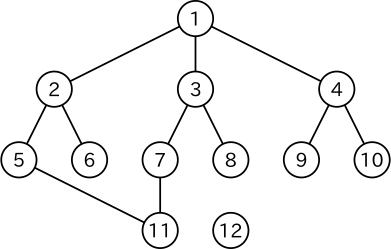
\includegraphics[width=.5\linewidth]{initial-tree-cycle-example.pdf}
    \caption{長さ6の閉路を含む,頂点数12,次数3の初期グラフ}
    \label{fig:initial-graph-cycle-example}
  \end{figure}
\end{example}

\section{全域木}
\label{sect:initial-spanning-tree}
\begin{conjecture}[全域木予想]
  \label{conj:spanning-tree}
  一般化ムーアグラフの誘導グラフには,次のような全域木が存在する.
\end{conjecture}
\begin{example}
  予想\ref{conj:spanning-tree}に従っていくつかの全域木を構築する.
  構築した初期グラフを図\ref{fig:initial-spanning-tree-example}に示す.
  \begin{figure}
    \centering
    \subfloat[頂点数$12$,次数$3$の全域木]{
      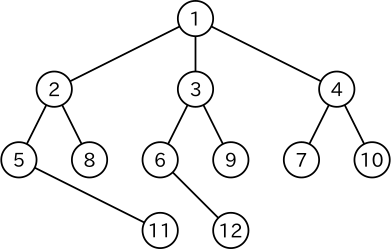
\includegraphics[width=.4\linewidth]
                      {initial-spanning-tree-12-example.pdf}
    }\hfill
    \subfloat[頂点数$18$,次数$3$の全域木]{
      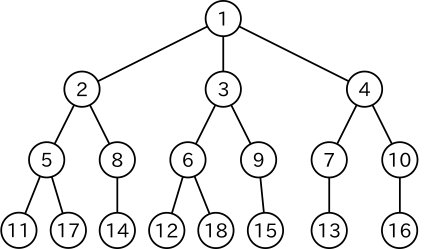
\includegraphics[width=.45\linewidth]
                      {initial-spanning-tree-18-example.pdf}
    }
    \caption{全域木の例}
    \label{fig:initial-spanning-tree-example}
  \end{figure}
\end{example}

\section{実験}
\label{sect:exp-reduce-by-initial}

\section{結果}
\label{sect:result-reduce-by-initial}


\chapter{枝刈りによる探索空間の削減}
\label{chap:reduce-by-prune}
枝刈りによって探索空間を削減する.
本稿では,直径の下界を計算し,定理\ref{thm:gmg-geometric-property}
の条件\ref{gmg-geom-b}を満足するか求めることで実現する.

\section{直径の下界の計算}
\label{sect:diameter-lower-bound}
直径の下界を計算する方法を与える.まず,次のグラフを定義する.
\begin{definition}
  探索途中のグラフ$G$と候補辺番号$i$に対するオペレータの適応を行う前とする.
  この状態について,グラフ$G$に候補辺番号$i$以降のすべての辺($E'=\{e_j\}_{j>i}$)
  を追加したグラフ$G+E'$を\textbf{最大グラフ}と定義する.
  このとき,最大グラフのもとになったグラフ$G$を\textbf{最小グラフ}と呼ぶ.
\end{definition}
\begin{example}
  図\ref{fig:min-max-graph}に最小グラフと最大グラフの例を示す.
  最小グラフの破線部分はオペレータ適応の判定が行われていない候補辺を表す.
  最大グラフは,最小グラフのオペレータ適応未決定の辺をすべて追加したグラフと
  なっている.
\end{example}
\begin{figure}
  \centering
  \subfloat[最小グラフ]{
    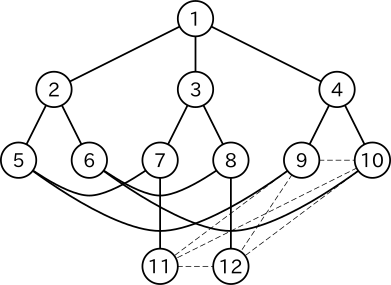
\includegraphics[width=.4\linewidth]
                    {min-graph-example.pdf}
  }\hfill
  \subfloat[最大グラフ]{
    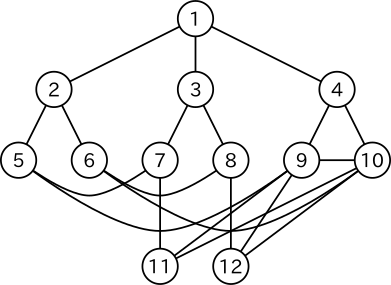
\includegraphics[width=.4\linewidth]
                    {max-graph-example.pdf}
  }
  \caption{最小グラフと最大グラフの例}
  \label{fig:min-max-graph}
\end{figure}
直径の下界は,最大グラフの直径を計算すればよい.もし直径の下界が
定理\ref{thm:gmg-geometric-property}の条件\ref{gmg-geom-b}を
満たさない場合,それ以降どのように辺を追加しても条件を満たさないので,
その場で探索を打ちきることができる.
この事実を応用して,一般化ムーアグラフの探索に直径の条件を考慮した
枝刈りを与える.探索で用いる状態は,最小グラフと最大グラフと候補辺の番号の
三つ組である.

次に,追加オペレータと無追加オペレータを新たに定めた状態に適応する.
追加オペレータは,最小グラフ$G_{\min}$と最大グラフ$G_{\max}$と候補辺番号$i$に
対して,最小グラフ$G'_{\min}=G_{\min}+e_i$と最大グラフ$G'_{\max}=G_{\max}$と
次の候補辺番号$i+1$を返す.また,無追加オペレータは,最小グラフ$G_{\min}$と
最大グラフ$G_{\max}$と候補辺番号$i$に対して,最小グラフ$G'_{\min}=G_{\min}$と
最大グラフ$G'_{\max}=G_{\max}-e_i$と次の候補辺番号$i+1$を返す.
さらに,系\ref{coll:basic-noadd-operator}で示した無追加オペレータの適応条件は
次のようになる.
\begin{corollary-without-proof}
  \label{coll:minmax-noadd-operator}
  無追加オペレータについて,与えられた最小グラフを$G_{\min}$,最大グラフを
  $G_{\max}$,候補辺番号を$i$,対象の辺を$e_i=\{v,w\}$とし,
  適応後の最小グラフを$G'_{\min}$,最大グラフを$G'_{\max}$とする.
  $i$以降の辺$\{e_j\}_{j>i}$の選び方次第で
  $G_{\min}'+E\,(E\subset \{e_j\}_{j>i})$が一般化ムーアグラフとなる見込み
  があることは,次の二条件を満たすことである.
  \begin{enumerate}
  \item 次数条件$\cdots$ $\text{Exit}(x)=i$なる$x\in e_i$について,
    $d_{G'_{\min}}(x)=k$.
  \item 直径条件$\cdots$ $G'_{\max}$の直径が定理\ref{thm:gmg-geometric-property}で
    示された直径以下である.
  \end{enumerate}
\end{corollary-without-proof}

最後に,枝刈りを適応した探索の手続きをアルゴリズム\ref{algo:minmax-algorithm}
に示す.これは,アルゴリズム\ref{algo:basic-algorithm}を書き換えるものである.
\begin{algorithm}[H]
  \caption{最大グラフを用いた一般化ムーアグラフの探索アルゴリズム}
  \label{algo:minmax-algorithm}
  \begin{algorithmic}[1]
    \Require $n,k$
    \Ensure $M(n,k)\:$(見つからない場合,$\varnothing$を返す)
    \Procedure{FindGeneralizedMooreGraph}{}
    \State $G_{I\min}\gets\text{初期グラフ}$
    \State $\{e_i\}_{i\in\mathbb{N}}^M\gets G_{I\min}\text{の候補辺}$
    \State $G_{I\max}\gets G_{I\min}+\{e_i\}$
    \Comment 初期グラフに対する最大グラフ
    \State $Stack\gets((G_{I\min},G_{I\max},1))$
    \While{$|Stack|>0$}
    \State $G_{\min},G_{\max},i\gets pop(Stack)$
    \If{$i>M$かつ
      $G_{\min}$が正則で定理\ref{thm:gmg-geometric-property}を満たす}
    \State \textbf{return} $G_{\min}$
    \EndIf
    \ForAll{$operator\in\{\text{無追加オペレータ},\text{追加オペレータ}\}$}
    \If{$operator$が$G_{\min},G_{\max},i$に適応できる}
    \Comment 系\ref{coll:basic-add-operator}と系\ref{coll:minmax-noadd-operator}
    \State $push(Stack,operator(G_{\min},G_{\max},i))$
    \EndIf
    \EndFor
    \EndWhile
    \State \textbf{return} $\varnothing$
    \EndProcedure
  \end{algorithmic}
\end{algorithm}

\section{頂点間距離の高速な更新法}
\label{sect:fast-distance-update}
\ref{sect:apply-to-gmg}節と\ref{sect:diameter-lower-bound}節にて,
グラフが一般化ムーアグラフになり得るかを判定するには,追加する辺に接続する
二つの頂点間距離と,直径の下界を求める必要があることを述べた.
本節では,これらの値を高速に計算するため,辺の挿入と削除に対して頂点間距離を
更新するアルゴリズムを与える.この方法の導入により,
探索空間の削減にはつながらないが,計算量が削減され実行時間の短縮が期待できる.

グラフ$G=(V,E),V=\{1,\ldots n\}$のすべての頂点の組$\{s,t\}$の距離$d(s,t)$と
距離が$d(s,t)$となる最短経路の数$\sigma(s,t)$が与えられているとする.
便宜上,$s=t$の場合はそれぞれ$d(s,s)=0,\,\sigma(s,s)=1$とする.
まず,$d(s,t)$と$\sigma(s,t)$について,追加と削除に共通するいくつかの
補題を示す.
\begin{lemma-without-proof}[Brandes\cite{Brandes2001}]
  \label{lemma:distance-1}
  $G=(V,E)$の異なる二頂点$s,t\in V$に対して,$s$から$t$への最短経路
  $G_{st}=(V_{st},E_{st})$が$v\in V$を含む,すなわち$v\in V_{st}$であるための
  必要十分条件は
  \[ d(s,t)=d(s,v)+d(v,t) \]
  が成り立つことである.
\end{lemma-without-proof}
\begin{lemma-without-proof}[難波ら\cite{Nanba2016}]
  \label{lemma:distance-2}
  $G=(V,E)$の異なる二頂点$s,t\in V$と辺$\{v,w\}\in E$を考える.
  $s$から$t$への最短経路$G_{st}=(V_{st},E_{st})$が辺$\{v,w\}$を含む,
  すなわち$\{v,w\}\in E_{st}$が成り立つための必要十分条件は
  \[ d(s,t)=d(s,v)+d(w,t)+1 \]
  が成り立つことである.ただし,$d(s,v)\leq d(s,w)$とする.
\end{lemma-without-proof}
\begin{lemma-without-proof}[Brandes\cite{Brandes2001}]
  \label{lemma:path-num-1}
  $G=(V,E)$の異なる二頂点$s,t\in V$に対して,$s$から$t$への最短経路の中で
  $v$を通るものの個数$\sigma_v(s,t)$は次式で与えられる.
  \[ \sigma_v(s,t)=\begin{aligned}\begin{cases}
    \sigma(s,v)\sigma(v,t) & d(s,t)=d(s,v)+d(v,t)\text{のとき} \\
    0 & \text{それ以外のとき}
  \end{cases}\end{aligned} \]
\end{lemma-without-proof}
\begin{lemma-without-proof}[難波ら\cite{Nanba2016}]
  \label{lemma:path-num-2}
  $G=(V,E)$の異なる二頂点$s,t\in V$に対して,$s$から$t$への最短経路の中で
  辺$\{v,w\}$を通るものの個数$\sigma_{vw}(s,t)$は次式で与えられる.
  \[ \sigma_{vw}(s,t)=\begin{aligned}\begin{cases}
    \sigma(s,v)\sigma(w,t) & d(s,t)=d(s,v)+d(w,t)+1\text{のとき} \\
    0 & \text{それ以外のとき}
  \end{cases}\end{aligned} \]
  ただし,$d(s,v)\leq d(s,w)$とする.
\end{lemma-without-proof}

次の補題は,ある二頂点間の最短経路の個数と,その経路に含まれる
短い最短経路の個数との関係を示す.
\begin{lemma}
  \label{lemma:number-of-paths}
  $G=(V,E)$の異なる二頂点$s,t\in V$について,$v$を$d(s,t)=d(s,v)+d(v,t)$
  である頂点(ただし$v\neq s,t$)とすると,次が成り立つ.
  \begin{equation}
    \label{eq:number-of-paths}
    \sigma(s,t)=\frac{\sum_{v}\sigma(s,v)\sigma(v,t)}{d(s,t)-1}
  \end{equation}
\end{lemma}
\begin{proof}
  $s$と$t$の間の一般的な経路を図\ref{fig:proof-number-of-paths}に示す.
  \begin{figure}
    \centering
    \def\svgwidth{.5\columnwidth}
    \input{proof-number-of-paths.pdf_tex}
    \caption{$s$と$t$の一般的な最短経路}
    \label{fig:proof-number-of-paths}
  \end{figure}
  $s$からの距離が一定の頂点を並べて,一つの層とする.$d(s,v)=k$なる頂点
  $v$の集合を,第$k$層と定義し,$L_k$と表す.
  $L_k$に属する頂点の数を$n_k$,$L_k$に属する$l$番目の頂点を$v_{kl}$と表す.
  ここで,第$k$層に属する頂点$v$は,隣接する層(第$k-1$層と第$k+1$層)
  以外の層に属する頂点$w$と隣接しないことに注意する.
  もしそのような頂点が存在すると,最短経路長が変化する.
  式\ref{eq:number-of-paths}の両辺に$d(s,t)-1$を掛けて,
  次の式\ref{eq:number-of-paths1}を得る.
  \begin{equation}
    \sigma(s,t)(d(s,t)-1)=\sum_{v}\sigma(s,v)\sigma(v,t)
    \label{eq:number-of-paths1}
  \end{equation}
  式\ref{eq:number-of-paths1}の右辺を,
  図\ref{fig:proof-number-of-paths}にならって表すと,
  \begin{equation}
    \sum_{v}\sigma(s,v)\sigma(v,t)=
    \sum_{k=1}^m\sum_{l=1}^{n_k}\sigma(s,v_{kl})\sigma(v_{kl},t)
    \label{eq:number-of-paths2}
  \end{equation}
  が得られる.ここで,二つの頂点$v$と$w$について,次の隣接を表す記号$a$を
  導入する.
  \begin{align*}
    a(v,w)=
    \begin{cases}
      1 & vとwが隣接しているとき \\
      0 & vとwが隣接していないとき
    \end{cases}
  \end{align*}
  各々の$\sigma(s,v_{kl})\sigma(v_{kl},t)$について議論する.
  $a$の定義を用いて式を変形すると,
  \begin{align}
    &\sigma(s,v_{kl})\sigma(v_{kl},t)\nonumber\\
    =&\left(\sum_{v'\in L_{k-1}}\sigma(s,v')a(v',v_{kl})\right)
    \left(\sum_{v'\in L_{k+1}}\sigma(v_{kl},v')a(v',t)\right)
    \nonumber\\
    =&\left(\sum_{v''\in L_{k-2}}\sum_{v'\in L_{k-1}}
    \sigma(s,v'')a(v'',v')a(v',v_{kl})\right)
    \left(\sum_{v'\in L_{k+1}}\sum_{v''\in L_{k+2}}
    a(v_{kl},v')a(v',v'')\sigma(v'',t)\right)
    \nonumber\\
    &\vdots\nonumber\\
    =&\left(\sum_{(v_1,\ldots,v_{k-1})\in L_1\times\cdots\times L_{k-1}}
    a(s,v_1)\cdots a(v_{k-1},v_{kl})\right)
    \left(\sum_{(v_{k+1},\ldots,v_m)\in L_{k+1}\times\cdots\times L_m}
    a(v_{kl},v_{k+1})\cdots a(v_m,v_t)\right)\nonumber\\
    =&\sum_{
      (v_1,\ldots,v_{k-1},v_{k+1},\ldots,v_m)\in
      L_1\times\cdots\times L_{k-1}\times L_{k+1}\times\cdots\times L_m
    }
    a(s,v_1)\cdots a(v_{k-1},v_{kl})a(v_{kl},v_{k+1})\cdots a(v_m,t)
    \label{eq:number-of-paths3}
  \end{align}
  が得られる.式\ref{eq:number-of-paths3}を式\ref{eq:number-of-paths2}に
  代入すると,
  \begin{align}
    &\sum_{k=1}^m\sum_{l=1}^{n_k}\sigma(s,v_{kl})\sigma(v_{kl},t)\nonumber\\
    =&\sum_{k=1}^m\sum_{l=1}^{n_k}\sum_{
      (v_1,\ldots,v_{k-1},v_{k+1},\ldots,v_m)\in
      L_1\times\cdots\times L_{k-1}\times L_{k+1}\times\cdots\times L_m
    }
    a(s,v_1)\cdots a(v_{k-1},v_{kl})a(v_{kl},v_{k+1})\cdots a(v_m,t)\nonumber\\
    =&\sum_{k=1}^m\sum_{(v_1,\ldots,v_m)\in L_1\times\cdots\times L_m}
    a(s,v_1)\cdots a(v_m,t)\nonumber\\
    =&m\left(\sum_{(v_1,\ldots,v_m)\in L_1\times\cdots\times L_m}
    a(s,v_1)\cdots a(v_m,t)\right)
    \label{eq:number-of-paths4}
  \end{align}
  と変形できる.式\ref{eq:number-of-paths4}の総和の対象が$1$となるのは,
  $a(s,v_1),\ldots,a(v_m,t)$のすべてが$1$のとき,
  すなわち,$s$と$v_1$,$v_1$と$v_2$,$\ldots$,$v_m$と$t$がすべて隣接している
  とき,すなわち,$s$と$t$の最短経路となっているときである.
  従って,総和の値は$s$と$t$の最短経路の数と一致し,
  式\ref{eq:number-of-paths4}は$\sigma(s,t)(d(s,t)-1)$と等しい.
  従って,補題が成り立つ.
\end{proof}

\subsection*{辺の挿入に対する頂点間距離の更新}
$G$に辺$e=\{\alpha,\beta\}\notin E(G)$を挿入したた後の頂点間距離$d'(s,t)$と
最短経路数$\sigma'(s,t)$を求める.
ここでは,難波ら\cite{Nanba2016}が提案した方法に関する重要な定理と
アルゴリズムを示す.
\begin{theorem-without-proof}[難波ら\cite{Nanba2016}]
  \label{thm:update-distance-on-insert}
  グラフ$G=(V,E)$から辺$\{\alpha,\beta\}\notin E$を追加した後の
  頂点間距離$d'(s,t)$と最短経路数$\sigma'(s,t)$について,次が成り立つ.
  ただし,$d(s,\alpha)\leq d(s,\beta)$とする.
  \begin{enumerate}
  \item $d(s,\alpha)<d(s,\beta)$かつ$d(s,t)>d(s,\alpha)+d(\beta,t)+1$ならば,
    次が成り立つ.
    \[ d'(s,t)=d(s,\alpha)+d(\beta,t)+1,\:
    \sigma'(s,t)=\sigma(s,\alpha)\sigma(\beta,t) \]
  \item $d(s,\alpha)<d(s,\beta)$かつ$d(s,t)=d(s,\alpha)+d(\beta,t)+1$ならば,
    次が成り立つ.
    \[ d'(s,t)=d(s,t),\:
    \sigma'(s,t)=\sigma(s,t)+\sigma(s,\alpha)\sigma(\beta,t) \]
  \item $d(s,\alpha)=d(s,\beta)$または$d(s,t)<d(s,\alpha)+d(\beta,t)+1$ならば,
    次が成り立つ.
    \[ d'(s,t)=d(s,t),\:\sigma'(s,t)=\sigma(s,t) \]
  \end{enumerate}
\end{theorem-without-proof}

定理\ref{thm:update-distance-on-insert}を元にして,
辺の挿入に対する$d(s,t)$と$\sigma(s,t)$の更新の手順を与える.
それをアルゴリズム\ref{algo:update-distance-on-insert}に示す.
\begin{algorithm}[H]
  \caption{辺$\{\alpha,\beta\}$が追加されたときの$d'(s,t)$と$\sigma'(s,t)$の
    更新}\label{algo:update-distance-on-insert}
  \begin{algorithmic}[1]
    \Require $G=(V,E),\,d(s,t),\,\sigma(s,t)$
    \Ensure $d'(s,t),\,\sigma'(s,t)$
    \ForAll{$(s,t)\in V\times V,\,s<t$}
    \State $(\alpha,\beta)$のうち$s$に近いほうを$\alpha$とする
    \If{$d(s,\alpha)<d(s,\beta)$かつ$d(s,t)>d(s,\alpha)+d(\beta,t)+1$}
    \State $d'(s,t)\gets d(s,\alpha)+d(\beta,t)+1$
    \State $\sigma'(s,t)\gets \sigma(s,\alpha)\sigma(\beta,t)$
    \ElsIf{$d(s,\alpha)<d(s,\beta)$かつ$d(s,t)=d(s,\alpha)+d(\beta,t)+1$}
    \State $d'(s,t)\gets d(s,t)$
    \State $\sigma'(s,t)\gets \sigma(s,t)+\sigma(s,\alpha)\sigma(\beta,t)$
    \ElsIf{$d(s,\alpha)=d(s,\beta)$または$d(s,t)<d(s,\alpha)+d(\beta,t)+1$}
    \State $d'(s,t)\gets d(s,t)$
    \State $\sigma'(s,t)\gets\sigma(s,t)$
    \Else
    \EndIf
    \EndFor
  \end{algorithmic}
\end{algorithm}

\subsection*{辺の削除に対する頂点間距離の更新}
$G$から辺$e=\{\alpha,\beta\}\in E(G)$を削除した後の頂点間距離$d'(s,t)$と
最短経路数$\sigma'(s,t)$を求める.次の定理が成り立つ.
\begin{theorem}
  \label{thm:update-distance-on-delete}
  グラフ$G=(V,E)$から辺$\{\alpha,\beta\}\in E$を削除した後の
  頂点間距離$d'(s,t)$と最短経路数$\sigma'(s,t)$について,次が成り立つ.
  ただし,$d(s,\alpha)\leq d(s,\beta)$とする.
  \begin{enumerate}
  \item $\sigma_{\alpha\beta}(s,t)=0$ならば,次が成り立つ.
    \[ d'(s,t)=d(s,t),\:\sigma'(s,t)=\sigma(s,t) \]
  \item $0<\sigma_{\alpha\beta}(s,t)<\sigma(s,t)$ならば,次が成り立つ.
    \[ d'(s,t)=d(s,t),\:\sigma'(s,t)=\sigma(s,t)-\sigma_{\alpha\beta}(s,t) \]
  \item $\sigma_{\alpha\beta}(s,t)=\sigma(s,t)>0$ならば,次が成り立つ.
    \begin{equation*}
      \begin{aligned}
        d'(s,t)&=\min\{d(s,v)+d(v,t)\,|\,v\in V,\,
        \sigma(s,v)>\sigma_{\alpha\beta}(s,v),\,
        \sigma(v,t)>\sigma_{\alpha\beta}(v,t) \\
        \sigma'(s,t)&=\frac{\sum_v(\sigma'(s,v)\sigma'(v,t))}{d'(s,t)-1}\:
        (v\in V,\,v\neq s,t,\,d'(s,t)=d'(s,v)+d'(v,t))
      \end{aligned}
    \end{equation*}
  \end{enumerate}
\end{theorem}
\begin{proof}
  辺削除による更新の操作は次の三種類である.
  \begin{enumerate}
  \item 削除による影響はなく,何も行わない
  \item 削除により最短経路数を更新する
  \item 削除により頂点間距離を更新し,さらに最短経路数を再計算する
  \end{enumerate}

  一つ目の操作が実施される場合は,辺$\{\alpha,\beta\}$が$s$と$t$との
  最短経路に含まれていないときである.これは,補題\ref{lemma:path-num-2}より,
  $\sigma_{\alpha\beta}(s,t)=0$のときと言い換えられる.

  二つ目の操作が実施される場合は,
  $s$と$t$との最短経路の集合$P\neq\varnothing$と,
  $P$の中で辺$\{\alpha,\beta\}$を含む経路の集合$P'\neq\varnothing$に対して,
  $P'\subset P$のときである.
  言い換えると,補題\ref{lemma:path-num-2}より,
  $0<\sigma_{\alpha\beta}(s,t)<\sigma(s,t)$のときである.
  このとき,削除により$P'$に属する最短経路がなくなるため,
  その数($\sigma_{\alpha\beta}(s,t)$)だけ$\sigma(s,t)$から引いた値とする.

  三つ目の操作が実施される場合は,
  $s$と$t$との最短経路の集合$P\neq\varnothing$と,
  $P$の中で辺$\{\alpha,\beta\}$を含む経路の集合$P'\neq\varnothing$に対して,
  $P'=P$のときである.
  言い換えると,補題\ref{lemma:path-num-2}より,
  $\sigma_{\alpha\beta}(s,t)=\sigma(s,t)>0$のときである.
  このとき,削除により$P$に属する最短経路がすべて無効になるため,頂点間距離を
  再計算する.補題\ref{lemma:distance-1}より,
  新しい頂点間距離$d'(s,t)$を計算できる.このとき,中間の頂点$v$は
  削除による頂点間距離の更新が起こらない頂点を選ぶ.
  また,新しい最短経路数$\sigma'(s,t)$は補題\ref{lemma:number-of-paths}により
  計算できる.
\end{proof}

定理\ref{thm:update-distance-on-delete}より,一辺削除時の頂点間距離の
更新の方法が分かる.
その手順ををアルゴリズム\ref{algo:update-distance-on-delete}に示す.
\begin{algorithm}[H]
  \caption{辺$\{\alpha,\beta\}$が削除されたときの$d'(s,t)$と$\sigma'(s,t)$の
    更新}\label{algo:update-distance-on-delete}
  \begin{algorithmic}[1]
    \Require $G=(V,E),\,d(s,t),\,\sigma(s,t)$
    \Ensure $d'(s,t),\,\sigma'(s,t)$
    \State $P\gets()$
    \Comment{更新の対象となる頂点組$(s,t)$}
    \ForAll{$(s,t)\in V\times V,\,s<t$}
    \If{$\sigma_{\alpha\beta}(s,t)=0$}
    \State $d'(s,t)=d(s,t)$
    \State $\sigma'(s,t)=\sigma(s,t)$
    \ElsIf{$0<\sigma_{\alpha\beta}(s,t)<\sigma(s,t)$}
    \State $d'(s,t)=d(s,t)$
    \State $\sigma'(s,t)=\sigma(s,t)-\sigma_{\alpha\beta}(s,t)$
    \ElsIf{$\sigma_{\alpha\beta}(s,t)=\sigma(s,t)>0$}
    \Comment{頂点間距離を再計算}
    \State $d_{\min}\gets \infty$
    \ForAll{$v\in V,\,
      \sigma(s,v)>\sigma_{\alpha\beta}(s,v),\,
      \sigma(v,t)>\sigma_{\alpha\beta}(v,t)$}
    \State $d_{\min}\gets\min\left\{d_{\min},d(s,v)+d(v,t)\right\}$
    \EndFor
    \If{$d_{\min}=\infty$}
    \State $d'(s,t)\gets\infty$
    \State $\sigma'(s,t)\gets0$
    \Else
    \State $d'(s,t)\gets d_{\min}$
    \State \parbox[t]{\linewidth}{
      $P\gets(\ldots,(s_i,t_i),(s,t),(s_{i+1},t_{i+1}),\ldots)$ \\
      ただし,$d'(s_i,t_i)\leq d'(s,t)\leq d'(s_{i+1},t_{i+1}),\:$
      $\ldots,(s_i,t_i),\ldots\in P$
    }
    \EndIf
    \EndIf
    \EndFor
    \ForAll{$(s_i,t_i)\in P$}
    \Comment{最短経路数を再計算}
    \State $\sigma'\gets0$
    \ForAll{$v\in V,\:v\neq s_i,t_i,\:d'(s_i,t_i)=d'(s_i,v)+d'(v,t_i)$}
    \State $\sigma'\gets\sigma'+\sigma'(s_i,v)\sigma'(v,t_i)$
    \EndFor
    \State $\sigma'(s_i,t_i)\gets\sigma'/(d'(s_i,t_i)-1)$
    \EndFor
  \end{algorithmic}
\end{algorithm}

アルゴリズム\ref{algo:update-distance-on-delete}では,頂点間距離の
再計算の対象の組$(s,t)$を$d'(s,t)$の昇順になるようにリストに追加している.
この根拠は次の系\ref{coll:update-distance-on-delete}で与える.
\begin{corollary}
  \label{coll:update-distance-on-delete}
  頂点間距離を再計算した組$(s,t)$について,最短経路数
  $\sigma'(s,t)$を再計算するには,すべての$d'(s,t)>d'(u,v)$なる
  $(u,v)$の$\sigma'(u,v)$を先に計算しなければならない.
\end{corollary}
\begin{proof}
  定理\ref{thm:update-distance-on-delete}の更新手順より,
  $s$と$t$の最短経路数の中に$d'(s,t)>d'(u,v)$なる$u$と$v$の最短経路数
  が含まれる.よって,$\sigma'(s,t)$を再計算するには,すべての
  $d'(s,t)>d'(u,v)$なる$(u,v)$の$\sigma'(u,v)$を先に計算しなければならない.
\end{proof}

\subsection*{一辺削除時の頂点間距離の更新の実験}
提案した手法が有効であることを検証するために,次の手順で実験を行う.
\begin{enumerate}
\item 削除前のグラフ$G=(V,E)$を構築する.グラフの種類はランダムネットワーク
  (Erd\H{o}s-R{\'e}nyiモデル\cite{Erdos1959})とスケールフリーネットワーク
  (Barab{\'a}si-Albertモデル\cite{Barabasi1999})の二種類とする.
\item $G$のすべての頂点の組$(s,t)\in[V]^2$に対して,
  頂点間距離$d(s,t)$と最短経路数$\sigma(s,t)$を求める.
  このとき,igraphライブラリの\verb|igraph_get_all_shortest_paths|
  を用いて求める.
\item 辺$\{\alpha,\beta\}\in E$をランダムに選ぶ.選んだ辺を削除した後の
  頂点間距離と最短経路数を二通りの方法で求め,計算に要した時間を計測する.
  \begin{enumerate}[a]
  \item (igraphライブラリ)\verb|igraph_shortest_paths|で求める
  \item (提案手法)アルゴリズム\ref{algo:update-distance-on-delete}で求める
  \end{enumerate}
\item 以上の手順を,ネットワーク種類とパラメータごとに100回繰り返し,
  計算に要した時間の平均を求める.
\end{enumerate}
ネットワークのパラメータは,頂点数は$10,50,100,300,600,1000,1500,2000$とし,
Erd\H{o}s-R{\'e}nyiモデルに対しては$p=0.1,0.3,0.6,0.9$とし,
Barab{\'a}si-Albertモデルに対しては$m=3,6,10,15,20$とする.

実験の実行環境は表\ref{tab:env-mws}のとおりである.
\begin{table}
  \caption{実行環境}
  \label{tab:env-mws}
  \centering
  \begin{tabular}{ll}
    \hline
    プロセッサ & Intel® Core™ i7-4712HQ CPU @ 2.30GHz × 4 \\ \hline
    メインメモリ & 3.9GiB \\ \hline
    ベースシステム & Ubuntu 16.04.3 LTS 64 ビット \\ \hline
    仮想化 & Oracle VirtualBox バージョン 5.1.18 r111374 \\ \hline
    コンパイラ & gcc 5.4.0 \\ \hline
    グラフライブラリ & igraph 0.7.1-2.1 \\ \hline
    最適化フラグ & -Ofast \\ \hline
  \end{tabular}
\end{table}

\subsubsection*{結果}
一辺削除時の頂点間距離の更新の実験結果を図\ref{fig:dist-delete}に示す.
図\ref{fig:dist-delete-igraph-random}にigraphライブラリとErd\H{o}s-R{\'e}nyiモデル
の結果を,
図\ref{fig:dist-delete-igraph-scalefree}にigraphライブラリと
Barab{\'a}si-Albertモデルの結果を,
図\ref{fig:dist-delete-proposed-random}に提案手法とErd\H{o}s-R{\'e}nyiモデル
の結果を,
図\ref{fig:dist-delete-proposed-scalefree}に提案手法と
Barab{\'a}si-Albertモデルの結果をそれぞれ示す.

図\ref{fig:dist-delete-igraph-random}と図\ref{fig:dist-delete-igraph-scalefree}
よりigraphライブラリでは$p$と$m$の増加による計算時間の増加が見られるが,
図\ref{fig:dist-delete-proposed-random}と
図\ref{fig:dist-delete-proposed-scalefree}より
提案手法ではそのような傾向は見られない.
このことから,提案手法は,頂点数に対して辺数が比較的多い密なグラフに対して
有効であることが確認できる.

\begin{figure}
  \centering
  \includegraphics{dist-delete-1-1.pdf}
  \includegraphics{dist-delete-1-2.pdf}
  \hspace{-5mm}
  \includegraphics{dist-delete-random-title.pdf}
  \hspace{5mm}
  \includegraphics{dist-delete-1-2.pdf}
  \hspace{-5mm}
  \includegraphics{dist-delete-scalefree-title.pdf}
  \includegraphics{dist-delete-1-1.pdf}
  \vspace{-3mm}

  \includegraphics{dist-delete-2-1.pdf}
  \includegraphics{dist-delete-2-2.pdf}
  \hspace{-5mm}
  \includegraphics{dist-delete-random-legend.pdf}
  \hspace{5mm}
  \includegraphics{dist-delete-2-2.pdf}
  \hspace{-5mm}
  \includegraphics{dist-delete-scalefree-legend.pdf}
  \includegraphics{dist-delete-2-1.pdf}
  \vspace{-3mm}

  \includegraphics{dist-delete-igraph-ylab.pdf}
  \includegraphics{dist-delete-igraph-random-yaxis.pdf}
  \hspace{-5mm}
  \subfloat[igraphライブラリ,Erd\H{o}s-R{\'e}nyiモデル]{
    \includegraphics{dist-delete-igraph-random.pdf}
    \label{fig:dist-delete-igraph-random}
  }\hspace{5mm}
  \includegraphics{dist-delete-igraph-scalefree-yaxis.pdf}
  \hspace{-5mm}
  \subfloat[igraphライブラリ,Barab{\'a}si-Albertモデル]{
    \includegraphics{dist-delete-igraph-scalefree.pdf}
    \label{fig:dist-delete-igraph-scalefree}
  }
  \includegraphics{dist-delete-3-6.pdf} \\
  \vspace{3mm}

  \includegraphics{dist-delete-proposed-ylab.pdf}
  \includegraphics{dist-delete-proposed-random-yaxis.pdf}
  \hspace{-5mm}
  \subfloat[提案手法,Erd\H{o}s-R{\'e}nyiモデル]{
    \includegraphics{dist-delete-proposed-random.pdf}
    \label{fig:dist-delete-proposed-random}
  }\hspace{5mm}
  \includegraphics{dist-delete-proposed-scalefree-yaxis.pdf}
  \hspace{-5mm}
  \subfloat[提案手法,Barab{\'a}si-Albertモデル]{
    \includegraphics{dist-delete-proposed-scalefree.pdf}
    \label{fig:dist-delete-proposed-scalefree}
  }
  \includegraphics{dist-delete-3-6.pdf}

  \caption{一辺削除時の頂点間距離の更新の比較}
  \label{fig:dist-delete}
\end{figure}

\section{実験}
\label{sect:exp-reduce-by-prune}
提案した枝刈りの有効性を検証するため,次の実験を行う.
枝刈りを導入する前の探索と\ref{sect:diameter-lower-bound}節で説明した枝刈りと
\ref{sect:fast-distance-update}節で説明した高速化に対して,次の指標を測定する
ことで比較を行う.
\begin{enumerate}
\item 最初の一般化ムーアグラフが発見されるまでの時間
\item 最初の一般化ムーアグラフが発見されるまでの展開状態数
\end{enumerate}
実験のパラメータは\ref{sect:exp-basic-algorithm}節で示したものと同じである.

さらに,\ref{sect:fast-distance-update}節で説明した高速化の効果を検証するため,
次の指標を用いて\ref{sect:diameter-lower-bound}節の枝刈りと比較する.
\begin{enumerate}\setcounter{enumi}{2}
\item 展開状態数に対する平均探索時間
\end{enumerate}
なお,用いる初期グラフは\ref{sect:initial-spanning-tree}節で説明した
全域木初期グラフとする.
この実験のパラメータは,頂点数を$n\leq30$,次数を$k=3,4$とする.
本節の実験の環境は,\ref{sect:exp-basic-algorithm}節で示したものと同じである.

\section{結果}
探索開始から最初の一般化ムーアグラフの発見までに要した探索時間を
図\ref{fig:sinitr-time}に示す.探索開始から最初の一般化ムーアグラフの発見までの
状態展開数を図\ref{fig:sinitr-state}に示す.さらに,展開状態数に対する
平均探索時間を図\ref{fig:sinitr-time-by-state}に示す.
図\ref{fig:sinitr-time}と図\ref{fig:sinitr-time-by-state}にて,
最大グラフとは,\ref{sect:diameter-lower-bound}節で示した枝刈りの方法を,
距離更新とは,\ref{sect:fast-distance-update}節で示した頂点間距離更新を
導入した方法を表す.

まず,枝刈りの導入の効果について考察する.
図\ref{fig:sinitr-state}より,枝刈りによって展開状態数が減少し,高効率化に
成功している.しかし,図\ref{fig:sinitr-time}より,枝刈りの導入によって
探索時間が増加するような頂点数と次数の組合せもある.これは,状態が二つのグラフを
保持しているために,プログラムが大量のグラフのデータの生成と破棄を繰り返すことに
よって,枝刈りでもたらされる高効率化に追いつかないことが原因と考えられる.
その根拠に,図\ref{fig:sinitr-state-d3}にて,頂点数が10のときは展開状態数が
少なくならないが,図\ref{fig:sinitr-time-d3}の頂点数が10のときは
探索時間が長くなっていることが考えられる.

次に,枝刈りの高速化について考察する.図\ref{fig:sinitr-time-by-state-d3}より,
$k=3$のときは距離更新の導入によって時間がかかることに対して,
図\ref{fig:sinitr-time-by-state-d4}より,$k=4$のときは距離更新の導入によって
わずかに高速に探索できることが分かる.理由として,距離更新の導入によって状態が
保持するデータが増加したこと(グラフ1個と$n\times n$行列が4個)により
状態の生成と削除に必要な時間が増加したことと,距離更新アルゴリズムは
密なグラフで有効であることの二つが考えられる.

\begin{figure}
  \centering
  \noindent\makebox[\textwidth]{
    \includegraphics{sinitr-time-lpad.pdf}
    \includegraphics{sinitr-time-ylab.pdf}
    \includegraphics{sinitr-time-d3-yaxis.pdf}\hspace{-3mm}
    \subfloat[$k=3$]{
      \includegraphics{sinitr-time-d3.pdf}
      \label{fig:sinitr-time-d3}
    }\hspace{5mm}
    \includegraphics{sinitr-time-d4-yaxis.pdf}\hspace{-3mm}
    \subfloat[$k=4$]{
      \includegraphics{sinitr-time-d4.pdf}
      \label{fig:sinitr-time-d4}
    }
    \includegraphics{sinitr-time-legend.pdf}
  }
  \caption{最初の一般化ムーアグラフの発見までの時間}
  \label{fig:sinitr-time}
\end{figure}

\begin{figure}
  \centering
  \noindent\makebox[\textwidth]{
    \includegraphics{sinitr-state-lpad.pdf}
    \includegraphics{sinitr-state-ylab.pdf}
    \includegraphics{sinitr-state-d3-yaxis.pdf}\hspace{-3mm}
    \subfloat[$k=3$]{
      \includegraphics{sinitr-state-d3.pdf}
      \label{fig:sinitr-state-d3}
    }\hspace{5mm}
    \includegraphics{sinitr-state-d4-yaxis.pdf}\hspace{-3mm}
    \subfloat[$k=4$]{
      \includegraphics{sinitr-state-d4.pdf}
      \label{fig:sinitr-state-d4}
    }
    \includegraphics{sinitr-state-legend.pdf}
  }
  \caption{最初の一般化ムーアグラフの発見までの展開状態数}
  \label{fig:sinitr-state}
\end{figure}

\begin{figure}
  \centering
  \noindent\makebox[\textwidth]{
    \includegraphics{sinitr-time-by-state-lpad.pdf}
    \includegraphics{sinitr-time-by-state-ylab.pdf}
    \includegraphics{sinitr-time-by-state-d3-yaxis.pdf}\hspace{-3mm}
    \subfloat[$k=3$]{
      \includegraphics{sinitr-time-by-state-d3.pdf}
      \label{fig:sinitr-time-by-state-d3}
    }\hspace{5mm}
    \includegraphics{sinitr-time-by-state-d4-yaxis.pdf}\hspace{-3mm}
    \subfloat[$k=4$]{
      \includegraphics{sinitr-time-by-state-d4.pdf}
      \label{fig:sinitr-time-by-state-d4}
    }
    \includegraphics{sinitr-time-by-state-legend.pdf}
  }
  \caption{展開状態数に対する平均探索時間}
  \label{fig:sinitr-time-by-state}
\end{figure}


\chapter{一般化ムーアグラフの列挙}
本章では,第\ref{chap:reduce-by-initial-graph}章で導入した初期グラフの
妥当性(予想\ref{conj:gmg-cycle}と予想\ref{conj:spanning-tree})を検証する.
そのために,一般化ムーアグラフを重複なく列挙する方法を与え,実験を行う.

\section{列挙アルゴリズム}
\label{sect:enum-algorithm}
一般化ムーアグラフを重複なく列挙する,つまり,非同型な一般化ムーアグラフを
列挙する方法を与える.同型なグラフとは,二つのグラフ$G=(V,E)$と$G'=(V',E')$が
与えられたとき,$G$と$G'$を一致させるような$V$のラベルの付け替え$g$
が存在することをいう.
\[ g:V\rightarrow V',g(V)=V',\{\{g(v),g(w)\}|e=\{v,w\}\in E\}=E' \]
非同型な一般化ムーアグラフを列挙する手順をアルゴリズム\ref{algo:gmg-enumeration}
に示す.ここで,$\text{Aut}(G)$をグラフ$G$の同型グラフの集合とする.

\begin{algorithm}[H]
  \caption{一般化ムーアグラフの列挙アルゴリズム}
  \label{algo:gmg-enumeration}
  \begin{algorithmic}[1]
    \Require $n,k$
    \Ensure 互いに非同型な$M(n,k)$の集合
    \Procedure{EnumerateGeneralizedMooreGraph}{}
    \State $G_I\gets\text{初期グラフ}$
    \State $\{e_i\}_{i\in\mathbb{N}}^M\gets G_I\text{の候補辺}$
    \State $Gs_1\gets\{G_I\}$
    \ForAll{$i\in\{1,\ldots,M\}$}
    \State $Gs_{i+1}\gets\varnothing$
    \ForAll{$G\in Gs_i$}
    \ForAll{$operator\in\{\text{追加オペレータ},\text{無追加オペレータ}\}$}
    \If{$G,e_i$に$operator$が適応でき,かつ,
      $operator(G,e_i)\notin\cup_{H\in Gs_{i+1}}\text{Aut}(H)$}
    \State $Gs_{i+1}\gets Gs_{i+1}\cup\{operator(G,e_i)\}$
    \EndIf
    \EndFor
    \EndFor
    \EndFor
    \State \textbf{return} $\{G\,|\,G\in Gs_{M+1},$
    $G\text{が正則で定理\ref{thm:gmg-geometric-property}を満たす}\}$
    \EndProcedure
  \end{algorithmic}
\end{algorithm}

\section{実験}
節\ref{sect:enum-algorithm}で定義したアルゴリズムを用いて,一般化ムーアグラフを
列挙し,第\ref{chap:reduce-by-initial-graph}章で導入した初期グラフの妥当性を
検証する.具体的には,初期グラフを変更してアルゴリズムを開始し,得られた
一般化ムーアグラフの個数が同じかを確認する.
検証する頂点数$n$と次数$k$は,$k=3,4$と
\begin{equation*}
  \begin{aligned}
    n=\begin{cases}
      4,6,8,10,12,14,16,18 & (k=3) \\
      5,6,7,8,9,10,11 & (k=4)
    \end{cases}
  \end{aligned}
\end{equation*}
とする.実験を行った環境は,表\ref{tab:env-lab}の通りである.

\section{結果}
アルゴリズムにより得られた一般化ムーアグラフの数を表\ref{tab:ginitr-ngraph-iso}
に示す.

% latex table generated in R 3.4.2 by xtable 1.8-2 package
% Thu Jan  4 15:06:44 2018
\begin{table}[ht]
\centering
\caption{初期グラフを変更したときの互いに非同型な一般化ムーアグラフの数} 
\label{tab:ginitr-ngraph-iso}
\begin{tabular}{lrrr}
  \hline
$(n,d)$ & 基本初期グラフ & 閉路初期グラフ & 全域木初期グラフ \\ 
  \hline
(4,3) &   1 &   1 &   1 \\ 
  (6,3) &   2 &   2 &   2 \\ 
  (8,3) &   2 &   2 &   2 \\ 
  (10,3) &   1 &   1 &   1 \\ 
  (12,3) &   2 &   2 &   2 \\ 
  (14,3) &   7 &   7 &   7 \\ 
  (16,3) &   6 &   6 &   6 \\ 
  (18,3) &   1 &   1 &   1 \\ 
  (5,4) &   1 &   1 &   1 \\ 
  (6,4) &   1 &   1 &   1 \\ 
  (7,4) &   2 &   2 &   2 \\ 
  (8,4) &   6 &   6 &   6 \\ 
  (9,4) &  16 &  16 &  16 \\ 
  (10,4) &  24 &  24 &  24 \\ 
  (11,4) &  37 &  37 &  37 \\ 
   \hline
\end{tabular}
\end{table}


結果のとおり,初期グラフを変更したことによって列挙されない一般化ムーアグラフは
存在しないことが分かる.つまり,実験を行った頂点数と次数の範囲では,
初期グラフの変更は妥当である.


\chapter{結論}
本論文では,深さ優先探索法を基にした一般化ムーアグラフの探索の高効率化に
ついて述べた.まず,一般化ムーアグラフの基本的性質を証明した.
次に,この性質を利用して,一般化ムーアグラフを探索するアルゴリズムを提案した.
最後に,探索空間の削減による高効率化の方法を提案し,その効果を実験によって示した.

本論文では,高効率化の方法として,探索の初期状態を変更することと
枝刈りの二つを提案した.
探索の初期状態の変更とは,初期状態のグラフに予めいくつかの辺を追加した状態を
新たな初期状態とすることである.本論文では,辺を二本追加して閉路を含むようにした
グラフと,全域木の二種類を提案した.実験の結果から,一般的な場合では全域木から
探索を始める場合が最も効率が良いことが分かった.また,閉路を含むグラフは
ある頂点数と次数の組合せにおいて,効率が悪くなることが示された.
また,枝刈りの方法として,探索途中のグラフの直径の下界を用いる方法を提案した.
枝刈りによって探索空間が削減され高効率化は達成されたが,
頂点数および次数が小さい場合に探索に時間がかかることが結果から示された.

今後の課題は,提案した方法を用いて一般化ムーアグラフの存在を調べることや,
提案した初期状態から探索を開始することの妥当性の証明,
および,一般化ムーアグラフが存在しないときの,平均頂点間距離最小の正則グラフの
研究である.


\chapter*{謝辞}
本論文は筆者が岡山大学工学部情報系学科に在籍中の研究結果をまとめたものである.
本研究を行うにあたり,ご指導を頂いた岡山大学大学院自然科学研究科産業創成工学専攻
高橋規一教授に深謝の意を表する.
また,情報数理工学研究室の皆様には,日常の議論を通して多くの知識や示唆を頂いた.
ここに謝意を表する.

\appendix
\chapter{gmg\_finder マニュアル}\label{chap-experimental-program}

一般化ムーアグラフを探索するためのライブラリ

\section*{依存ライブラリ・ソフトウェア}\label{ux4f9dux5b58ux30e9ux30a4ux30d6ux30e9ux30eaux30bdux30d5ux30c8ux30a6ux30a7ux30a2}

\begin{itemize}
\tightlist
\item
  \texttt{gcc}
\item
  \texttt{makefile}
\item
  \texttt{igraph}
\item
  \texttt{python} (一部)
\end{itemize}

\section*{実験プログラム}\label{ux5b9fux9a13ux30d7ux30edux30b0ux30e9ux30e0}

プログラムをビルドするには,\texttt{git}で
\texttt{https://github.com/y-satotani/gmg-finder}をクローンする.
すべての実験は\texttt{src/experiment}ディレクトリに含まれている.
\texttt{src}ディレクトリで\texttt{make\ ;\ make\ install}を実行すると,
以下の実行ファイルが\texttt{bin}ディレクトリに生成される.

\begin{itemize}
\tightlist
\item
  \texttt{exp\_cmp\_algo.out}
\item
  \texttt{exp\_cmp\_algo\_full.out}
\item
  \texttt{exp\_dist\_delete.out}
\item
  \texttt{exp\_miner.out}
\item
  \texttt{exp\_cmp\_algo\_enum.out}
\item
  \texttt{exp\_enumer.out}
\end{itemize}

以下,各プログラムを順番に説明する.

\subsection*{\texorpdfstring{\texttt{exp\_cmp\_algo.out}}{exp\_cmp\_algo.out}}\label{expux5fcmpux5falgo.out}

初期グラフと枝刈りの方法を変えて,性能を測定する.
実行例と結果例は以下のとおり.

\begin{verbatim}
src> experiment/exp_cmp_algo.out basic basic basic 10 3
\end{verbatim}

\begin{verbatim}
10,3,2,0,150,basic,basic,basic,150,15,16,0.000144
\end{verbatim}

結果は,次の値が\texttt{,}で区切られている.

\begin{itemize}
\tightlist
\item
  頂点数
\item
  次数
\item
  \texttt{Q} (\texttt{gmgf::graph\_config::Q()})
\item
  \texttt{R} (\texttt{gmgf::graph\_config::R()})
\item
  頂点間距離の総和の下界
\item
  グラフ初期化子
\item
  \texttt{basic}=\texttt{gmgf::basic\_graph\_initr}
\item
  \texttt{cycle}=\texttt{gmgf::cycle\_graph\_initr}
\item
  \texttt{stree}=\texttt{gmgf::stree\_graph\_initr}
\item
  候補辺ソート
\item
  \texttt{basic}=ソートなし
\item
  \texttt{sorted}=\texttt{gmgf::sorted\_graph\_initr}でソート
\item
  状態初期化子
\item
  \texttt{basic}=\texttt{gmgf::basic\_state\_initr}
\item
  \texttt{minmax}=\texttt{gmgf::minmax\_state\_initr}
\item
  \texttt{matrix}=\texttt{gmgf::mmmtr\_state\_initr}
\item
  結果のグラフの頂点間距離の総和
\item
  候補辺の数
\item
  展開した状態数
\item
  実行時間 (\texttt{gmgf::dfs\_finder::next()}の実行時間)
\end{itemize}

次のコマンドで,複数の結果を含むcsvファイルを生成できる.
\texttt{-\/-max-procs=x}の\texttt{x}の値だけ並列に実行する.

\begin{verbatim}
(echo n,d,Q,R,sspl_lb,ginitr,sorted,sinitr,sspl,edge,node,time ;\
 ./exp_cmp_algo_param.py |\
 xargs --max-lines=1 --max-procs=4 ./exp_cmp_algo.out) >\
cmp-algo.csv
\end{verbatim}

パラメータは,\texttt{exp\_cmp\_algo\_param.py}で生成される.
別のパラメータで実験する場合は,このファイルを編集する.

\subsection*{\texorpdfstring{\texttt{exp\_cmp\_algo\_full.out}}{exp\_cmp\_algo\_full.out}}\label{expux5fcmpux5falgoux5ffull.out}

\texttt{exp\_cmp\_algo.out}では探索開始から(もしあれば)最初の一個の
一般化ムーアグラフを得るまでの情報を計測したが,
\texttt{exp\_cmp\_algo\_full.out}では探索開始からすべての一般化ムーアグラフ
を得るまでの情報を計測する.

\begin{verbatim}
./exp_cmp_algo_full.out basic basic basic 10 3
\end{verbatim}

の実行例は次のとおり.

\begin{verbatim}
10,3,2,0,150,basic,basic,basic,4,150,150,15,75,0.00042
\end{verbatim}

結果は,次の値が\texttt{,}で区切られている.

\begin{itemize}
\tightlist
\item
  頂点数
\item
  次数
\item
  \texttt{Q} (\texttt{gmgf::graph\_config::Q()})
\item
  \texttt{R} (\texttt{gmgf::graph\_config::R()})
\item
  頂点間距離の総和の下界
\item
  グラフ初期化子 (\texttt{exp\_cmp\_algo.out}と同じ)
\item
  候補辺ソート (\texttt{exp\_cmp\_algo.out}と同じ)
\item
  状態初期化子 (\texttt{exp\_cmp\_algo.out}と同じ)
\item
  結果のグラフの頂点間距離の総和
\item
  得られたグラフの数 (同型グラフを重複して数える)
\item
  最大の頂点間距離
\item
  最小の頂点間距離
\item
  候補辺の数
\item
  展開した状態数
\item
  実行時間
\end{itemize}

\subsection*{\texorpdfstring{\texttt{exp\_dist\_delete.out}}{exp\_dist\_delete.out}}\label{expux5fdistux5fdelete.out}

一辺削除時の頂点間距離の更新の実験を行う.次の項目を入力とする.

\begin{itemize}
\tightlist
\item
  ネットワークトポロジ
\item
  random=Erd\H{o}s--R{\'e}nyiモデル
\item
  scale-free=Barab{\'a}si--Albertモデル
\item
  頂点数
\item
  ネットワークパラメータ
\item
  シード値 (ランダム関数の)
\end{itemize}

\begin{verbatim}
./exp_dist_delete.out random 1000 0.3 0
\end{verbatim}

の実行例は以下のとおり.

\begin{verbatim}
1000,0.3,random,0,150422,1,0.827778,0.076536
\end{verbatim}

結果は次の値が\texttt{,}で区切られている.

\begin{itemize}
\tightlist
\item
  頂点数
\item
  ネットワークパラメータ (トポロジにより,pかm)
\item
  ネットワークトポロジ
\item
  \texttt{random}=Erd\H{o}s--R{\'e}nyiモデル
\item
  \texttt{scale-free}=Barab{\'a}si--Albertモデル
\item
  シード値
\item
  辺の数
\item
  結果が一致したかどうか (1なら一致)
\item
  \texttt{igraph}ライブラリでの計算時間
\item
  提案手法の計算時間
\end{itemize}

\subsection*{\texorpdfstring{\texttt{exp\_miner.out}}{exp\_miner.out}}\label{expux5fminer.out}

\texttt{exp\_cmp\_algo.out}で,グラフ初期化子を\texttt{gmgf::stree\_graph\_initr},
状態初期化子を\texttt{gmgf::minmax\_state\_initr}とし,
さらに(もしあれば)一般化ムーアグラフを出力する機能を付加したプログラム.

\begin{verbatim}
./exp_miner.out 10 3
\end{verbatim}

の実行例は以下のとおり,

\begin{verbatim}
10,3,2,0,150,150,15,16,0.000452
\end{verbatim}

結果は次の値が\texttt{,}で区切られている.

\begin{itemize}
\tightlist
\item
  頂点数
\item
  次数
\item
  \texttt{Q} (\texttt{gmgf::graph\_config::Q()})
\item
  \texttt{R} (\texttt{gmgf::graph\_config::R()})
\item
  頂点間距離の総和の下界
\item
  結果のグラフの頂点間距離の総和
\item
  候補辺の数
\item
  展開した状態数
\item
  実行時間 (\texttt{gmgf::dfs\_finder::next()}の実行時間)
\end{itemize}

さらに,\texttt{n\textless{}頂点数\textgreater{}-d\textless{}次数\textgreater{}-miner.elist}の形式で,一般化ムーアグラフの
辺リストを保存する.

\subsubsection*{\texorpdfstring{\texttt{exp\_miner.py}}{exp\_miner.py}}\label{expux5fminer.py}

\texttt{exp\_miner.out}に並列計算とタイムアウト機能を追加したプログラム.
コマンドライン引数は以下のとおり.

\begin{itemize}
\tightlist
\item
  \texttt{-n}=頂点数((次数+1)\ldots{}Nの範囲を対象とする)
\item
  \texttt{-d}=次数(3\ldots{}Dの範囲を対象とする)
\item
  \texttt{-i}=結果ファイルリスト(これらの結果に含まれている頂点数次数組は計算しない)
\item
  \texttt{-o}=結果ファイル(指定しなければ標準出力)
\item
  \texttt{-t}=タイムアウト時間(単位:秒)
\end{itemize}

結果は,\texttt{exp\_miner.out}の結果を列としたcsvファイルである.

\subsection*{\texorpdfstring{\texttt{exp\_cmp\_algo\_enum.out}}{exp\_cmp\_algo\_enum.out}}\label{expux5fcmpux5falgoux5fenum.out}

初期グラフと枝刈りの方法を変えて,互いに非同型な一般化ムーアグラフを列挙する.
実行例と結果例は以下のとおり.

\begin{verbatim}
src> experiment/exp_cmp_algo_enum.out basic basic basic 10 3
\end{verbatim}

\begin{verbatim}
10,3,2,0,150,basic,basic,basic,1,1,15,23,0.030401
\end{verbatim}

結果は,次の値が\texttt{,}で区切られている.

\begin{itemize}
\tightlist
\item
  頂点数
\item
  次数
\item
  \texttt{Q} (\texttt{gmgf::graph\_config::Q()})
\item
  \texttt{R} (\texttt{gmgf::graph\_config::R()})
\item
  頂点間距離の総和の下界
\item
  グラフ初期化子
\item
  \texttt{basic}=\texttt{gmgf::basic\_graph\_initr}
\item
  \texttt{cycle}=\texttt{gmgf::cycle\_graph\_initr}
\item
  \texttt{stree}=\texttt{gmgf::stree\_graph\_initr}
\item
  候補辺ソート
\item
  \texttt{basic}=ソートなし
\item
  \texttt{sorted}=\texttt{gmgf::sorted\_graph\_initr}でソート
\item
  状態初期化子
\item
  \texttt{basic}=\texttt{gmgf::basic\_state\_initr}
\item
  \texttt{minmax}=\texttt{gmgf::minmax\_state\_initr}
\item
  \texttt{matrix}=\texttt{gmgf::mmmtr\_state\_initr}
\item
  列挙されたすべてのグラフの頂点間距離の総和が下界に一致したか
\item
  列挙されたグラフの数
\item
  候補辺の数
\item
  展開した状態数
\item
  実行時間 (\texttt{gmgf::fbs\_enumer::enumerate()}の実行時間)
\end{itemize}

\texttt{exp\_cmp\_algo\_enum\_param.py}を用いて,複数のパラメータで実験することが
できる.方法は\texttt{exp\_cmp\_algo.out}の項を参照のこと.

\subsection*{\texorpdfstring{\texttt{exp\_enumer.out}}{exp\_enumer.out}}\label{expux5fenumer.out}

\texttt{exp\_cmp\_algo\_enum.out}で,グラフ初期化子を\texttt{gmgf::stree\_graph\_initr},
状態初期化子を\texttt{gmgf::minmax\_state\_initr}とし,
さらに,列挙された一般化ムーアグラフを出力する機能を付加したプログラム.

\begin{verbatim}
./exp_enumer.out 10 3
\end{verbatim}

の実行例は以下のとおり,

\begin{verbatim}
10,3,2,0,150,1,1,15,22,0.00152
\end{verbatim}

結果は次の値が\texttt{,}で区切られている.

\begin{itemize}
\tightlist
\item
  頂点数
\item
  次数
\item
  \texttt{Q} (\texttt{gmgf::graph\_config::Q()})
\item
  \texttt{R} (\texttt{gmgf::graph\_config::R()})
\item
  頂点間距離の総和の下界
\item
  列挙されたグラフすべての頂点間距離の総和が下界に一致したか
\item
  列挙されたグラフの数
\item
  候補辺の数
\item
  展開した状態数
\item
  実行時間 (\texttt{gmgf::fbs\_enumer::enumerate()}の実行時間)
\end{itemize}

さらに,\texttt{n\textless{}頂点数\textgreater{}-d\textless{}次数\textgreater{}-g\textless{}グラフ番号\textgreater{}-enumer.elist}の形式で,
一般化ムーアグラフの辺リストを保存する.

\subsubsection*{\texorpdfstring{\texttt{exp\_enumer.py}}{exp\_enumer.py}}\label{expux5fenumer.py}

\texttt{exp\_enumer.out}に並列計算とタイムアウト機能を追加したプログラム.
コマンドライン引数は以下のとおり.

\begin{itemize}
\tightlist
\item
  \texttt{-n}=頂点数((次数+1)\ldots{}Nの範囲を対象とする)
\item
  \texttt{-d}=次数(3\ldots{}Dの範囲を対象とする)
\item
  \texttt{-i}=結果ファイルリスト(これらの結果に含まれている頂点数次数組は計算しない)
\item
  \texttt{-o}=結果ファイル(指定しなければ標準出力)
\item
  \texttt{-t}=タイムアウト時間(単位:秒)
\end{itemize}

結果は,\texttt{exp\_enumer.out}の結果を列としたcsvファイルである.


\chapter{一般化ムーアグラフのリスト}
\label{chap:list-of-gmg}
付録\ref{chap-experimental-program}で説明した\verb|exp-miner.out|を
用いて,与えられた頂点数と次数の組の一般化ムーアグラフが存在するかを
求めた.その結果を図\ref{fig:gmg-existence}に示す.
ただし,予想\ref{conj:spanning-tree}の結果次第で,存在しない組が無効になる
可能性があることに注意する.ちなみに,一般化ムーアグラフの実体は,次の
URLにて公開している.

\url{github.com/y-satotani/gmg-finder/tree/master/docs/res/graph}

\begin{figure}[htbp]
  \centering
  \captionsetup{justification=centering}
  \includegraphics{gmg-existence-v.pdf}
  \caption{頂点数と次数の一般化ムーアグラフの存在\\
    空白部分は,正則グラフが存在しない組合せもしくは,
    まだ終了していない組合せを表す.}
  \label{fig:gmg-existence}
\end{figure}


\bibliography{../res/MyCollection}

\end{document}
